\documentclass[11pt,a4paper,oldfontcommands]{memoir}
\usepackage[utf8]{inputenc}
\usepackage[T1]{fontenc}
\usepackage{microtype}
\usepackage[dvips]{graphicx}
\usepackage{xcolor}
\usepackage{times}
\usepackage{float}
\usepackage[french]{babel}
\usepackage{listings}
\usepackage[normalem]{ulem}
\useunder{\uline}{\ul}{}

\usepackage[
breaklinks=true,colorlinks=true,
%linkcolor=blue,urlcolor=blue,citecolor=blue,% PDF VIEW
linkcolor=black,urlcolor=black,citecolor=black,% PRINT
bookmarks=true,bookmarksopenlevel=2]{hyperref}

\usepackage{geometry}
% PDF VIEW
% \geometry{total={210mm,297mm},
% left=25mm,right=25mm,%
% bindingoffset=0mm, top=25mm,bottom=25mm}
% PRINT
\geometry{total={210mm,297mm},
left=20mm,right=20mm,
bindingoffset=10mm, top=25mm,bottom=25mm}

% Hide appendix sections
\usepackage[toc,page]{appendix}
\usepackage{etoolbox}
\appto\appendix{\addtocontents{toc}{\protect\setcounter{tocdepth}{0}}}

\OnehalfSpacing
%\linespread{1.3}

%%% CHAPTER'S STYLE
\chapterstyle{bianchi}
%\chapterstyle{ger}
%\chapterstyle{madsen}
%\chapterstyle{ell}
%%% STYLE OF SECTIONS, SUBSECTIONS, AND SUBSUBSECTIONS
\setsecheadstyle{\Large\bfseries\sffamily\raggedright}
\setsubsecheadstyle{\large\bfseries\sffamily\raggedright}
\setsubsubsecheadstyle{\bfseries\sffamily\raggedright}
\setlength{\parskip}{1em}

%%% STYLE OF PAGES NUMBERING
\pagestyle{plain}
\makepagestyle{plain}
\makeevenfoot{plain}{\thepage}{}{}
\makeoddfoot{plain}{}{}{\thepage}
\makeevenhead{plain}{}{}{}
\makeoddhead{plain}{}{}{}
\maxsecnumdepth{subsubsection}
\maxtocdepth{subsection}

\begin{document}

\begin{titlepage}

\newcommand{\HRule}{\rule{\linewidth}{0.5mm}}

\center
 
%----------------------------------------------------------------------------------------
%	HEADING SECTIONS
%----------------------------------------------------------------------------------------

\textsc{\LARGE Haute École d'ingénierie et de gestion \\du canton de Vaud}\\[1.5cm]
\textsc{\Large Projet de groupe (PDG)}\\[0.5cm]
\textsc{\large Rapport de projet}\\[0.5cm]

%----------------------------------------------------------------------------------------
%	TITLE SECTION
%----------------------------------------------------------------------------------------

\HRule \\[0.8cm]
{ \huge \bfseries DrawTable}\\[0.4cm]
\HRule \\[1.5cm]
 
%----------------------------------------------------------------------------------------
%	AUTHOR SECTION
%----------------------------------------------------------------------------------------

\begin{minipage}{0.4\textwidth}
\begin{flushleft} \large
\emph{Auteurs:}\\
Sacha \textsc{Bron}\\
David \textsc{Villa}\\
Paul \textsc{Ntawuruhunga}\\
Yassin \textsc{Kammoun}\\
Marc \textsc{Pellet}
\end{flushleft}
\end{minipage}
~
\begin{minipage}{0.4\textwidth}
\begin{flushright} \large
\emph{Superviseur:} \\
Dr. René \textsc{Rentsch}
\break 
\break 
\break 
\break 
\end{flushright}
\end{minipage}\\[4cm]

%----------------------------------------------------------------------------------------
%	DATE SECTION
%----------------------------------------------------------------------------------------

{\large \today}\\[3cm]

%----------------------------------------------------------------------------------------
%	LOGO SECTION
%----------------------------------------------------------------------------------------


\includegraphics[scale=0.3]{images/heigvd.png}
\hfill

\includegraphics[scale=0.6]{images/hesso.png}

\vfill
\end{titlepage}

\cleardoublepage
\tableofcontents*
\cleardoublepage
\listoffigures*
\cleardoublepage
\listoftables*
\cleardoublepage

%----------------------------------------------------------------------------------------
%	INTRODUCTION
%----------------------------------------------------------------------------------------

\chapter{Introduction}

Ce chapitre se veut être une introduction de ce rapport de travail. Il s'agit dans un premier temps de rappeler le sujet du projet par une description complète de celui-ci. Viennent ensuite l'énumération, le commentaire et l'explication des objectifs que cherche à atteindre ce projet. Les technologies utilisées pour la réalisation du système sont introduites par la suite. Les différents membres constituant l'équipe de projet sont présentés. Cette introduction décrit précisément les rôles de chacun des protagonistes. Finalement, un commentaire quant à la décision de choisir un tel sujet de projet est exposé. Cela consiste à partager les motivations et les raisons qui ont poussé le groupe à partir sur un tel projet.

\section{Description du projet}

Le projet consiste en un outil de dessin tout à fait standard. Celui-ci permet entre autres de dessiner sur un espace de travail. Pour ce faire, l'utilisateur dispose d'un éventail d'outils:

\begin{itemize}
\item[$\bullet$] Outils de dessin: les outils de dessin mettent à disposition un crayon et une gomme permettant de dessiner sans restriction n'importe quelle forme géométrique.
\item[$\bullet$] Outils de formes: les outils de formes mettent à disposition un ensemble de formes géométriques prédéfinies pouvant être dessinées au sein d'un dessin et redimensionnées à la guise de l'utilisateur.
\item[$\bullet$] Outils de couleurs: les outils de couleurs mettent à disposition une palette de couleurs laquelle permet de définir la couleur du trait aussi bien pour les outils de dessin que pour les outils de formes.
\item[$\bullet$] Outils d'épaisseur: les outils d'épaisseur permettent de définir selon une liste prédéfinie l'épaisseur du trait aussi bien pour les outils de dessin que pour les outils de formes.
\end{itemize}

Malgré ce côté simpliste du système, celui-ci se démarque des outils de dessin traditionnels par le fait que l'espace de travail du dessinateur est non pas l'écran de l'utilisateur mais un support physique tel un mur, un sol, une table ou n'importe quelle autre surface susceptible de jouer le rôle de support de dessin. L'idéal est bien évidemment une surface plane. Toutefois, le système n'est pas restreint par une telle propriété. Celle-ci pourrait tout aussi bien être théoriquement abrupte, instable et biscornue. L'utilisateur définit lui-même ce qu'il juge être un support de dessin propice pour travailler.

\newpage

Le fait de dessiner sur un support physique plutôt que virtuel nécessite une substitution de la souris de l'ordinateur à un outil plus adéquat pour dessiner. Ceci est rendu possible par la mise à disposition d'un stylet au dessinateur. Ce stylet est conçu sur mesure par l'équipe de projet pour les besoins du système. Il reste toutefois un outil expérimental avec une casquette de prototype. En effet, celui-ci n'a pour but que de valider la conception et l'implémentation du système. Il n'en demeure pas moins que ce stylet reste relativement complexe pour accomplir une telle tâche.

Le stylet se présente sous la forme d'un stylo tout à fait usuel. Toutefois, de par l'objectif de son utilisation, il est caractérisé par les composants suivants:

\begin{itemize}
\item[$\bullet$] Une LED rouge.
\item[$\bullet$] Une LED verte.
\item[$\bullet$] Un interrupteur.
\item[$\bullet$] Une résistance.
\item[$\bullet$] Une batterie.
\item[$\bullet$] Un boîtier.
\end{itemize}

Bien que l'action de dessiner soit réalisée sur un support physique, le dessin à proprement parlé n'est pas gravé sur ce support. Les faits et gestes du dessinateur avec le stylet sont capturés par une caméra. Un programme informatique reçoit en permanence en provenance de cette caméra des informations liées aux faits et gestes du stylet manipulé par le dessinateur. C'est là qu'intervient le mécanisme du tracking, c'est-à-dire la détection et le suivi du stylet. Toutes ces informations récupérées sont communiqués à un autre programme informatique. Ce dernier stocke, analyse, traite et reproduit ces mêmes faits et gestes de manière à reconstituer logiquement et graphiquement le dessin correspondant.

Afin que le dessinateur puisse disposer d'un retour instantané de son dessin, un projecteur projette la reproduction fidèle du dessin réalisée au sein du second programme informatique. Ainsi, le dessinateur a l'illusion de dessiner directement sur son support physique. Il dispose en plus de cela des fonctionnalités usuelles de sérialisation de dessin. Il peut en effet enregistrer son travail et le reprendre ultérieurement.

La figure suivante illustre un exemple d'environnement de dessin :

\begin{figure}[h]
\centering
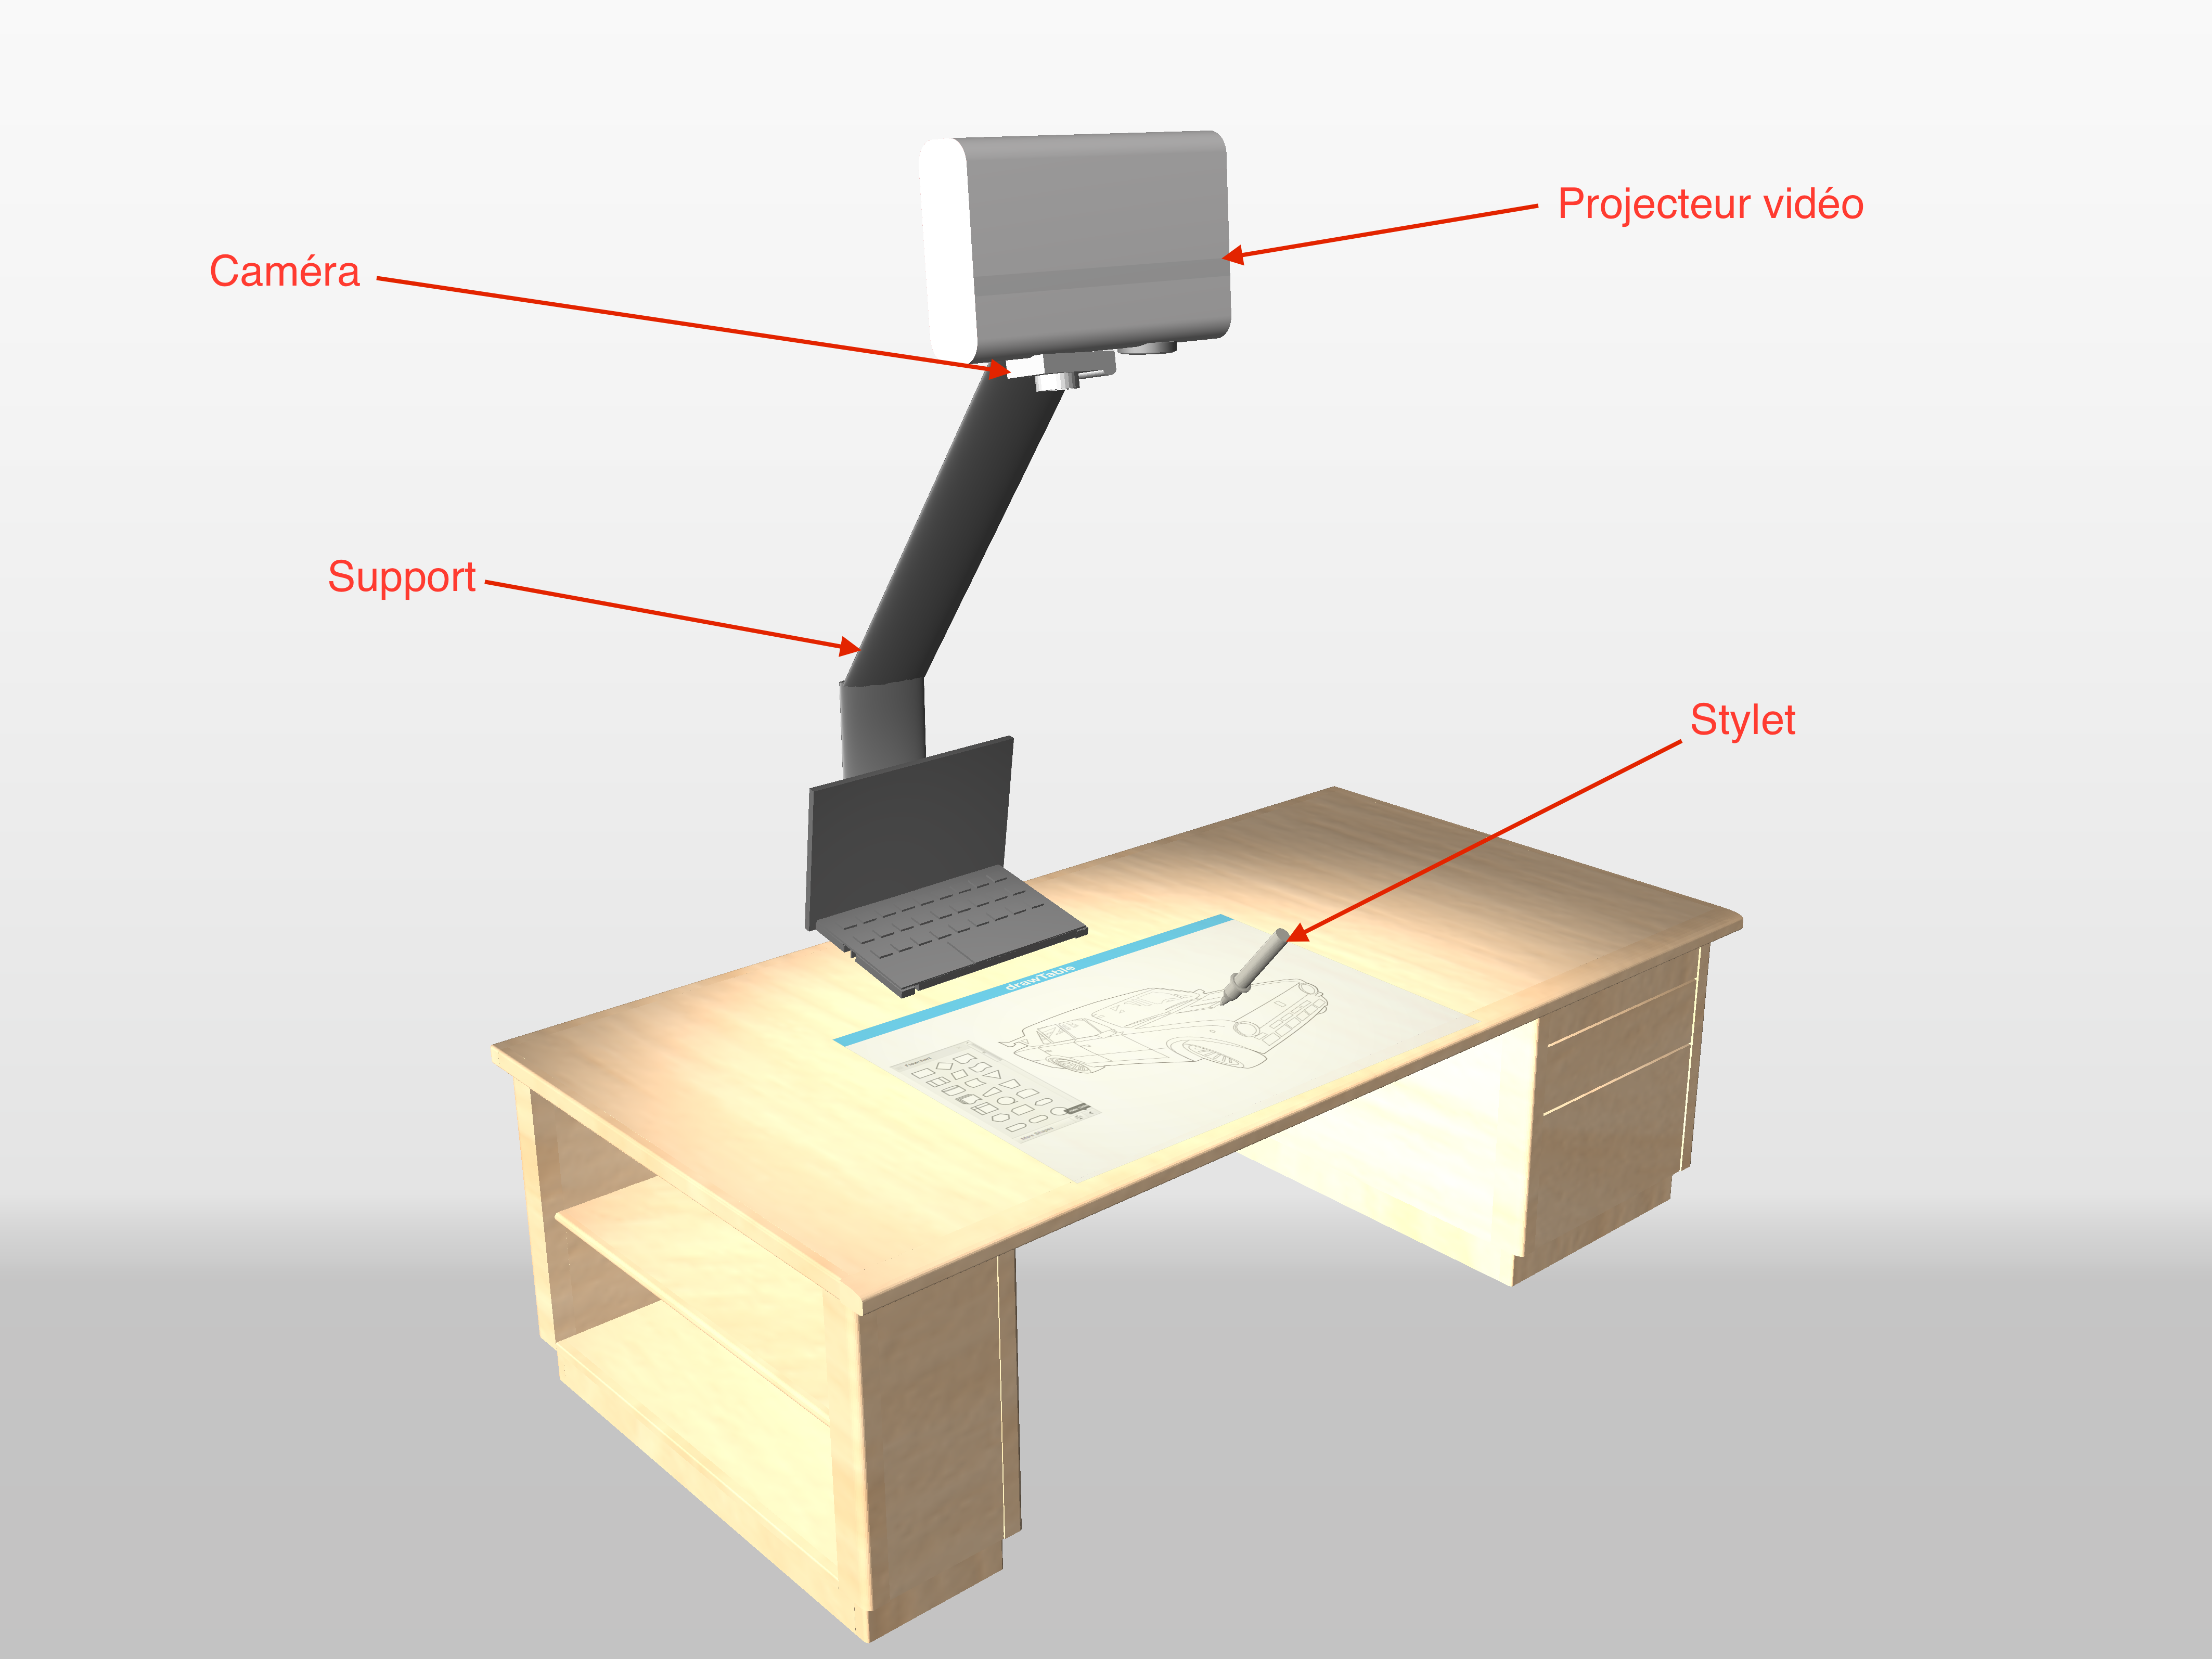
\includegraphics[scale=0.055]{images/drawing-environment.png}
\caption{Exemple d'environnement de dessin}
\end{figure}

\newpage

\section{Objectif du projet}

L'objectif de ce projet est de concevoir un outil de dessin assisté par ordinateur permettant à l'utilisateur de réaliser ses dessins de la manière la plus naturelle possible. À terme, l'utilisateur dessinera directement sur sa table ou n'importe quelle autre surface plane à l'aide d'un stylet et son dessin sera projeté sur son plan de travail, donnant ainsi à l'utilisateur l'impression de dessiner avec un crayon et une feuille.

\section{Technologies utilisées}

Les technologies utilisées pour le développement de l'application et le suivi du stylet sont les suivantes:

\begin{itemize}
\item[$\bullet$] Qt 5.5: Le framework Qt est une API orientée objet offrant des composants d'interface graphique, d'accès aux données, de connexions réseaux, de gestion des fils d'exécution, \dots. Dans le cadre du projet, elle est utilisée pour construire l'interface graphique utilisateur de l'application. Pour de plus amples informations, veuillez-vous référer au site officiel \url{http://www.qt.io}.
\item[$\bullet$] OpenCV 3.1: Open Computer Vision (OpenCV) est une bibliothèque graphique libre spécialisée dans le traitement d'images en temps réel. La bibliothèque OpenCV met à disposition de nombreuses fonctionnalités pour le traitement d'images, le traitement vidéos, les calculs matriciels, \dots. Dans le cadre du projet, elle est notamment utilisée pour le tracking du stylet. Pour de plus amples informations, veuillez-vous référer au site officiel \url{http://opencv.org}.
\item[$\bullet$] C++11: Le C++ est utilisé en guise de langage de programmation de base permettant de manipuler les différentes librairies utilisées dans le cadre du développement du projet. La librairie OpenCV et le framework Qt utilisant par défaut le langage C++, celui-ci constitue donc un choix idéal pour le développement du système.
\end{itemize}

\section{Équipe de projet}

Le tableau suivant présente l'équipe de projet, la hiérarchie au sein du groupe ainsi que les rôles joués par les différents membres du groupe:

\begin{table}[h]
\centering
\begin{tabular}{|l|l|c|l|}
\hline
\multicolumn{1}{|c|}{\textbf{Nom, prénom}} & \multicolumn{1}{c|}{\textbf{E-mail}} & \textbf{Hiérarchie}                 & \multicolumn{1}{c|}{\textbf{Rôles}} \\ \hline
Bron, Sacha                                & sacha.bron@heig-vd.ch                & \multicolumn{1}{l|}{Chef de projet} & TODO                                    \\ \hline
Villa, David                               & david.villa@heig-vd.ch               & \multicolumn{1}{l|}{Chef suppléant} & TODO                                    \\ \hline
Kammoun, Yassin                            & yassin.kammoun@heig-vd.ch            & -                                   & TODO                                    \\ \hline
Ntawuruhunga, Paul                         & paul.ntawuruhunga@heig-vd.ch         & -                                   & TODO                                    \\ \hline
Pellet, Marc                               & marc.pellet@heig-vd.ch               & -                                   & TODO                                    \\ \hline
\end{tabular}
\caption{Équipe de projet}
\end{table}

\section{Cadre de réalisation}

Ce projet s'inscrit dans le cadre du cours de Projet de Groupe (PDG) au sein de la Haute École d'ingénierie et de gestion du canton de Vaud (Heig-VD) sis à Yverdon-les-Bains. Selon le plan d'études de l'école, il est dispensé aux étudiants IL du département des Technologies de l'Information et de la Communication (TIC) pour le compte de leur troisième année de formation Bachelor. Le but de ce cours est d’effectuer un projet en passant par toutes les étapes de développement. Cela inclut le choix d'un sujet, la définition d’un cahier des charges, une phase de recherche et d'analyse suivie du développement de l’application et d’une phase de tests et de validation. En dernière instance, un rapport sur le déroulement du travail et une présentation du projet sont requis dans le but d'évaluer le travail effectué.

\section{Choix du sujet}

Le choix d'un tel sujet se justifie par le fait que ce projet exige un important travail de recherche, de découverte et d'apprentissage de nouvelles technologies comme cela peut notamment être le cas pour la librairie OpenCV. Bien évidemment, ce genre de projet présente des risques compte tenu du fait que la technologie n'est connue de personne, qu'elle peut être difficile à appréhender, à mettre en oeuvre et à maîtriser, que la faisabilité du projet n'est pas facilement définissable et que le temps d'apprentissage est difficilement estimable. Toutefois, toutes ces problématiques ne rendent le projet que plus motivant, attrayant et intéressant.

Ce projet s'inscrivant dans un cadre académique, il s'agit donc d'une opportunité idéale d'acquérir de nouvelles connaissances. Le sujet en lui-même est des plus intéressants. Il se démarque clairement de la monotonie des applications développées dans un tel contexte. Des projets similaires ont certainement déjà été réalisés que ce soit dans un cadre professionnel que dans un cadre académique mais à bien moindre mesure ce qui laisse énormément de place pour la créativité et l'innovation. Par ailleurs, la complexité d'un tel projet ne rend que plus grand le mérite une fois le travail terminé avec un système tout à fait fonctionnel.

D'un point de vue organisationnel, ce projet présente la particularité d'être subdivisé en deux sous-projets étant donné que deux programmes sont développés: l'outil de dessin et le système de tracking du stylet. Un troisième sous-projet pourrait encore ressortir de ces deux derniers puisque la conception et la fabrication du stylet est un travail à part entière. Ainsi, un défi clairement établi de ce projet est l'intégration des différentes composantes pour finalement former un tout.

En dernière instance, ce sujet de projet a été choisi en premier lieu par son originalité puisque il s'avère fort différent des travaux réalisés dans le cadre de la formation Bachelor. Par ailleurs, le fait qu'il présente une difficulté certaine et un risque potentiel d'échec rend le projet d'autant plus motivant à réaliser. Enfin, l'étude d'une nouvelle technologie telle que la librairie OpenCV jusque-là parfaitement inconnue à l'équipe est attrayante puisqu'elle permet à chaque membre du groupe d'enrichir son bagage technique.

%----------------------------------------------------------------------------------------
%	CONCEPTION
%----------------------------------------------------------------------------------------

\chapter{Conception}

Ce chapitre se veut être une description complète aussi bien de la conception du système que de la conception du stylet. L'architecture débute le descriptif du système par la présentation et la description de ses différentes composantes. Un diagramme de classes concis représentant l'ensemble du système est introduit. Viennent ensuite les présentations des deux composantes logicielles du système: le mécanisme de tracking et l'outil de dessin. Chacune fait l'objet d'une description plus approfondie de son architecture tout comme leur diagramme de classes respectif. Une décomposition de leur structure interne est effectuée de manière à décrire de manière indépendante le rôle et le fonctionnement de chaque constituant du système donné. Le stylet pour sa part est introduit en premier lieu par une description de son principe d'utilisation. Une présentation des différents composants matériels qui le constitue est ensuite réalisée. Un exposé du prototype de stylet est effectué au moyen de schémas. Les étapes de fabrication de celui-ci sont énumérées et commentées en long et large par la suite. Enfin, le fonctionnement du stylet est introduit. En dernière instance, l'environnement de dessin idéal est schématisé à l'aide de modélisations accompagnées de descriptions.

\section{Système global}

Cette section présente le système global du projet. Il s'agit d'exposer, de décrire et de commenter son architecture globale d'une part. D'autre part, il s'agit d'introduire le diagramme de classes correspondant. Celui-ci est toutefois concis dans la mesure où seules les entités sont mentionnées, ni méthode ni attribut n'y figurent dans le but bien évidemment d'alléger le contenu du schéma.

Le système met en jeu différents composants. Certains de ces composants sont de l'ordre du logiciel; d'autres sont de l'ordre du matériel. Cela se justifie par le fait que ce projet met non seulement en jeu différents composants de nature diverse mais en plus, ces composants sont supposés interagir et ce, malgré leur nature.

La relation entre composants peut prendre différentes formes. Certains composants interagissent entre eux par le biais d'une communication réseau. Certains encore utilisent des périphériques pour rediriger de l'information vers une sortie matérielle donnée. D'autres encore exploitent une entrée matérielle d'autres dispositifs pour récupérer des données.

\newpage

\subsection{Architecture}

La figure suivante présente l'architecture globale du système. Elle met en évidence entre autres les différentes composantes constituant le système:

\begin{figure}[h]
\centering
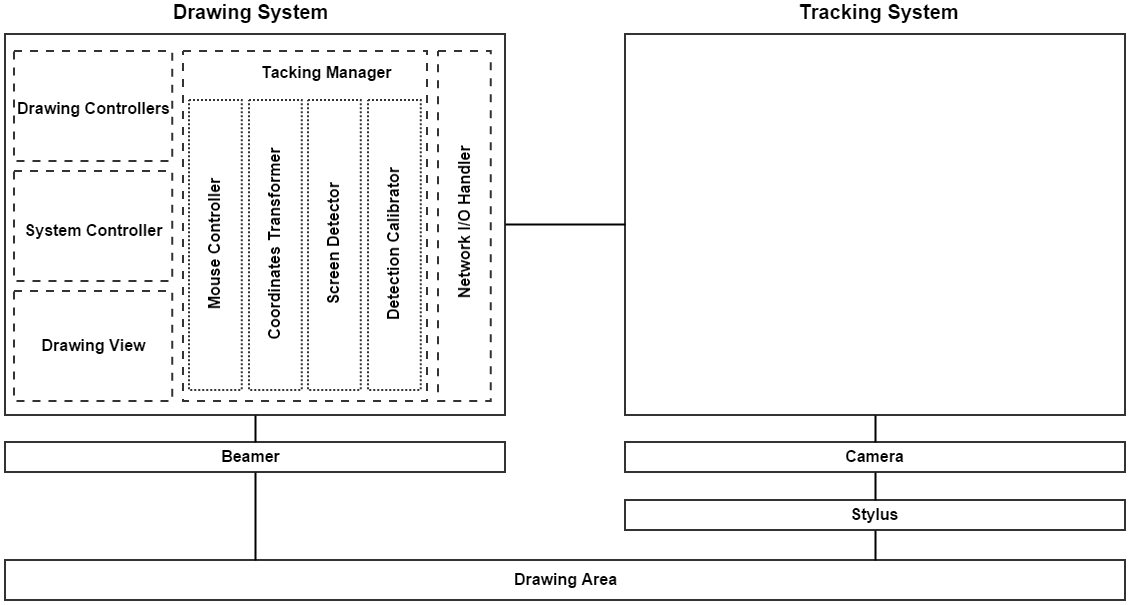
\includegraphics[scale=0.55]{images/global-system-architecture.png}
\caption{Architecture globale du système}
\end{figure}

\textit{TODO: décrire l'architecture globale du système.}

\subsection{Diagramme d'activités}

\textit{TODO: définir et décrire un diagramme d'activités mettant en jeu les différentes composants du système (Drawing System, Tracking System, Beamer, Drawing Area, Camera, Stylus).}

\subsection{Diagramme de classes}

\textit{TODO: définir et décrire le diagramme de classes de l'ensemble du système (avec entités, sans méthodes, sans attributs, sans cardinalités).}

\newpage

\section{Système de tracking}

\textit{TODO: introduire le contenu de la section (qu'est-ce qui y sera présenté dans l'ordre).}

\subsection{Architecture}

\textit{TODO: décrire l'architecture du système de tracking.}

\subsection{Diagramme d'activités}

\textit{TODO: définir et décrire un diagramme d'activités mettant en jeu le système de tracking (Tracking System), les constituants de sa structure interne, le système de dessin (Drawing System), la caméra (Camera), le stylet (Stylus) et le support de dessin (Drawing Area).}

\subsection{Diagramme de classes}

\textit{TODO: définir et décrire le diagramme de classes complet du système de tracking (avec entités, avec attributs, avec méthodes, avec cardinalités).}

\newpage

\section{Système de dessin}

Cette section présente le système de dessin. Il s'agit d'exposer, de décrire et de commenter son architecture d'une part. D'autre part, il s'agit d'introduire le diagramme de classes correspondant. Contrairement à celui du système global, le diagramme de classes ici est complet: attributs, méthodes, cardinalités et toute autre information jugée pertinente y figurent. Enfin, la structure interne du système y est décomposée. Chacune de ses constituantes y est décrite de manière indépendante.

Le système de dessin correspond à un outil logiciel lequel fournit une interface graphique utilisateur destinée à y produire virtuellement du dessin. Celui-ci a pour but de représenter logiquement et graphiquement sur un moniteur le dessin qu'un utilisateur est en train de dessiner sur son support physique qui, pour rappel, est supposé être n'importe quelle surface plane.

Cet outil de dessin a également pour objectif de fournir à l'utilisateur un ensemble de fonctionnalités lui permettant de manipuler son dessin. Ainsi, il se voit offrir un éventail d'outils:

\begin{itemize}
\item[$\bullet$] Outils de dessin:
    \begin{itemize}
    \item crayon, gomme.
    \end{itemize}
\item[$\bullet$] Outils de formes:
    \begin{itemize}
    \item cercle, rectangle.
    \end{itemize}
\item[$\bullet$] Outils de couleurs:
    \begin{itemize}
    \item palette de couleurs.
    \end{itemize}
\item[$\bullet$] Outils d'épaisseur:
    \begin{itemize}
    \item épaisseur de trait.
    \end{itemize}
\end{itemize}

Outre les fonctionnalités de dessin, l'outil se doit de proposer les fonctionnalités usuelles d'un logiciel dans la mesure où il s'agit d'une application manipulant un document, c'est-à-dire une unité d'informations lisible et susceptible d'être stockée de manière persistante. Dans le cas présent, il s'agit d'un dessin. Ainsi, les fonctions d'importation et de sauvegarde, d'impression et d'historique d'actions se doivent d'être disponibles, donc conçues et implémentées.

Selon ce qui a été défini dans le cahier des charges, les fonctionnalités suivantes sont donc mises à disposition dans l'application de dessin:

\begin{itemize}
\item[$\bullet$] Sérialisation:
    \begin{itemize}
    \item enregistrement, importation, impression.
    \end{itemize}
\item[$\bullet$] Historique d'actions:
    \begin{itemize}
    \item annulation, rétablissement.
    \end{itemize}
\end{itemize}

Compte tenu du fait que le système de dessin est susceptible de communiquer avec d'autres composantes du système global, notamment des composantes matérielles, des fonctionnalités supplémentaires se révèlent être nécessaires. Il s'agit notamment de permettre à l'utilisateur de pouvoir configurer les composantes matérielles interagissant avec les composantes logicielles de manière à ce qu'elles puissent fonctionner et communiquer de manière optimale avec les meilleurs paramètres possibles et donc, avec le meilleur taux de performance.

\newpage

\subsection{Architecture}

La figure suivante présente l'architecture du système de dessin:

\begin{figure}[h]
\centering
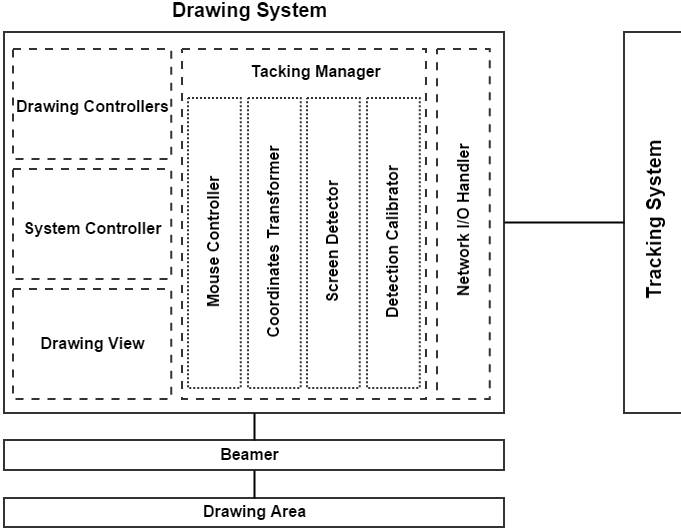
\includegraphics[scale=0.7]{images/drawing-system-architecture.png}
\caption{Architecture du système de dessin}
\label{fig:dsa}
\end{figure}

Le système de dessin est composé d'un certain nombre de constituants, chacun réalisant des tâches bien déterminées. Par ailleurs, le système de dessin fait l'objet d'une dépendance avec le système de tracking. En effet, ceux-ci interagissent ensemble par le biais d'une communication réseau.

La communication réseau avec le système de tracking est gérée du point de vue du système de dessin par un gestionnaire de communication réseau, symbolisé par le bloc \textit{Network I/O Handler} sur la figure \ref{fig:dsa}. Ce gestionnaire se comporte à la manière d'un \textit{listener}, d'un écouteur d'événements qui dans le cas présent consistent en la réception de messages. Ainsi, il se voit écouter tous les messages émis par le composant réseau du système de tracking. Les informations qui lui sont communiquées consistent typiquement en la description abstraite des faits et gestes de l'utilisateur avec le stylet sur le support physique, c'est-à-dire le bloc \textit{Drawing Area}. Cette description correspond typiquement en des actions survenues à des coordonnées données. Lors de la réception de tels messages, le gestionnaire de communication réseau transmet ces informations au gestionnaire de tracking du système de dessin, symbolisé par le bloc \textit{Tracking Manager} sur la figure \ref{fig:dsa}.

Le bloc \textit{Tracking Manager} remplit plusieurs rôles. Concrètement, il accomplit les tâches suivantes:

\begin{itemize}
\item[$\bullet$] Simuler la souris: il s'agit de simuler et de reproduire avec la souris de l'ordinateur les faits et gestes de l'utilisateur avec le stylet. Cela est assuré par le bloc \textit{Mouse Controller}.
\item[$\bullet$] Transformer des coordonnées: il s'agit de transformer les coordonnées du point de vue de la caméra vers le point de vue de l'écran. Cela est assuré par le bloc \textit{Coordinates Transformer}.
\item[$\bullet$] Détecter la projection d'écran: il s'agit de détecter la zone physique sur laquelle la projection de la reproduction du dessin est réalisée. Cela est réalisé par le biais du bloc \textit{Screen Detector}.
\item[$\bullet$] Calibrer la détection: il s'agit de calibrer la détection du stylet sur le support physique, c'est-à-dire de le localiser de manière précise en vue de l'exécution du mécanisme de tracking du stylet. Cette calibration est effectuée par le bloc \textit{Detection Calibrator}.
\end{itemize}

En définitive, le gestionnaire du tracking veille d'une part à ce que les composantes matérielles du système soient disponibles et fonctionnent de la manière la plus optimale possible. D'autre part, ce même gestionnaire tente tant bien que mal de reproduire ce que cherche à dessiner l'utilisateur en simulant ces faits et gestes et en les reportant sur l'équivalent logique du support physique de dessin.

L'ensemble des constituants du système de dessin est géré par un contrôleur général, ou contrôleur système, symbolisé par le bloc \textit{System Controller} sur la figure \ref{fig:dsa}. Celui-ci fait office de médiateur entre les différents constituants et veille à transmettre des messages lorsque besoin se fait sentir. Concrètement, il délègue à un constituant donné une tâche émise par un autre constituant. Ce contrôleur général est donc le noyau central du système de dessin, le coeur du système dit autrement.

Différents outils sont mis à la disposition de l'utilisateur en vue de dessiner et de personnaliser ses esquisses. Pour ce faire, différents contrôleurs sont définis de manière à traiter les interactions de l'utilisateur avec un outil donné. En conséquence, il y a autant de contrôleurs de dessin que d'outils prévus pour dessiner. Ces contrôleurs de dessin, ou contrôleurs d'outils de dessin, sont représentés par le bloc \textit{Drawing Controllers}. Ceux-ci sont mis à disposition du contrôleur général, \textit{System Controller} autrement dit.

Lorsque le contrôleur de souris, c'est-à-dire le bloc \textit{Mouse Controller}, simule une action utilisateur, celle-ci est émise au contrôleur général qui délègue la reproduction du geste de l'utilisateur selon l'outil utilisé au contrôleur de dessin approprié. Cette délégation est réalisée de manière abstraite. Le contrôleur général ne sait en aucun cas quel contrôleur de dessin se voit confier la tâche d'appliquer le geste utilisateur sur l'équivalent logique du dessin physique.

La reproduction des faits et gestes de l'utilisateur à l'aide du simulateur de souris, du contrôleur général et d'un contrôleur de dessin adéquat nécessite de disposer d'une vue sur laquelle ce traitement peut avoir lieu. Ceci est rendu possible par la définition d'une vue de dessin, symbolisée par le bloc \textit{Drawing View} sur la figure \ref{fig:dsa}. Le dessin que cherchera à dessiner l'utilisateur sera logiquement stocké dans ce constituant, affiché graphiquement et donc visible sur le moniteur de l'utilisateur. C'est précisément un des contrôleurs du bloc \textit{Drawing Controllers} qui effectuera cette tâche à la demande du contrôleur général, \textit{System Controller}, qui lui, aura réagi initialement à la demande du simulateur de souris, \textit{Mouse Controller}, qui aura reçu antérieurement une instruction de la part du système de tracking.

Le bloc \textit{Beamer} est un composant matériel à part entière. C'est vers celui-ci qu'est projetée la reproduction du dessin de l'utilisateur. D'un point de vue global de l'ensemble de l'infrastructure, le système n'accomplit aucune tâche pour que cette projection soit possiblement effective. Ce composant fait bel et bien partie du système dans la mesure où il reçoit indirectement de l'information en provenance d'un composant logiciel, le système de dessin en l'occurrence. Toutefois, cette transmission d'information n'est pas réalisée par le système présenté mais par le système d'exploitation de la machine hôte. Ainsi, il incombe à l'utilisateur de veiller à ce qu'un tel périphérique soit connecté à la machine hôte et qu'il soit opérationnel. En dernière instance, pour que la projection soit visible, il est attendu de l'utilisateur qu'il duplique ou qu'il étende son écran sur la sortie du projecteur de manière à ce que ce dernier affiche le contenu du moniteur.

Du point de vue du système de dessin, le bloc \textit{Drawing Area} n'est rien de plus qu'une zone sur laquelle est projetée la reproduction du dessin de l'utilisateur par le bloc \textit{Beamer}. Il s'agit tout simplement du support physique de l'utilisateur lequel remplace le support papier traditionnel.

\subsection{Diagramme d'activités}

\subsection{Diagramme de classes}

\subsection{Gestionnaire de communication réseau}

\subsection{Gestionnaire de tracking}

\subsubsection{Contrôleur de souris}

\subsubsection{Transformateur de coordonnées}

\subsubsection{Détecteur d'écran}

\subsubsection{Mécanisme de calibration}

\subsection{Contrôleur système}

\newpage

\subsection{Contrôleurs de dessin}

L'utilisation d'un outil de dessin nécessite le recours à un contrôleur adéquat devant permettre d'appliquer l'action que représente l'outil en question. Ainsi, dans le cas où l'utilisateur utiliserait la gomme, le contrôleur gérant la gomme devrait reproduire à l'exactitude les faits et gestes de l'utilisateur avec le stylet qui, dans le cas présent, représenterait une gomme.

\subsubsection{Hiérarchie des contrôleurs}

Les contrôleurs d'outils se présentent en plusieurs exemplaires. Chaque contrôleur a pour but de traiter les interactions de l'utilisateur avec son dessin pour un outil donné. Ainsi, si l'utilisateur manipule la gomme, le contrôleur relatif à la gomme entrera en scène et réagira aux actions de l'utilisateur, c'est-à-dire d'effacer là où l'utilisateur le demande. En l'occurrence, il s'agit du contrôleur nommé \textit{EraserController}. Si l'utilisateur manipule le crayon, le contrôleur relatif au crayon entrera en scène et ainsi de suite. Pour ce faire, une hiérarchie de contrôleurs d'outils a été établie. Elle est décrite par la figure suivante:

\begin{figure}[h]
\centering
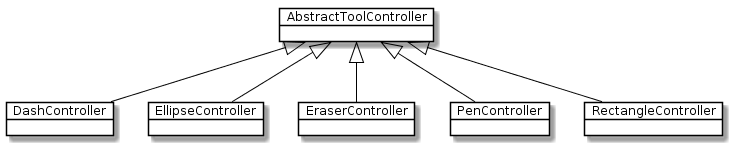
\includegraphics[scale=0.7]{images/tools-controllers-hierarchy.png}
\caption{Hiérarchie des contrôleurs d'outils}
\end{figure}

Un contrôleur d'outil abstrait est défini au sommet de la hiérarchie. Celui-ci apporte une couche d'abstraction à l'architecture dans la mesure où le contrôleur général ne sait à aucun moment avec quel contrôleur d'outil il interagit. Ainsi, lorsqu'un contrôleur est soumis à une tâche, le contrôleur général lui déléguera le travail. Par polymorphisme, la bonne implémentation du contrôleur d'outil sera appelée.

À noter qu'il y a autant de spécialisations de contrôleur d'outil qu'il y a d'outils mis à disposition de l'utilisateur. Pour rappel, les outils se présentent en quatre catégories à savoir les outils de dessin, les outils de formes, les outils de couleurs et les outils d'épaisseur. Toutefois, seules les deux premières font l'objet de contrôleurs d'outils, la raison étant due au fait que les outils appartenant à celles-ci sont les seuls permettant de produire du dessin à proprement parlé. Les autres font plutôt offices de cosmétiques pouvant être appliquées au dessin. Compte tenu de la hiérarchie établie et selon ce qui a été dit plus tôt, le mapping établi entre outils et contrôleurs d'outils se présente comme suit:

\begin{table}[h]
\centering
\begin{tabular}{|l|l|}
\hline
\multicolumn{1}{|c|}{\textbf{Outil}} & \multicolumn{1}{c|}{\textbf{Contrôleur d'outil}} \\ \hline
Crayon                               & PenController                                    \\ \hline
Gomme                                & EraserController                                 \\ \hline
Ligne                                & DashController                                   \\ \hline
Cercle                               & EllipseControler                                 \\ \hline
Rectangle                            & RectangleController                              \\ \hline
\end{tabular}
\caption{Mapping outil - contrôleur d'outil}
\end{table}

Bien que non représenté au sein de la figure précédente, les différents contrôleurs d'outil sont régis par les mêmes comportements. Ceux-ci sont effectivement appelés à réagir aux événements suivants:

\begin{itemize}
\item[$\bullet$] Mouvement de la souris.
\item[$\bullet$] Pression du bouton de la souris.
\item[$\bullet$] Relâchement du bouton de la souris.
\item[$\bullet$] Double-click de la souris.
\end{itemize}

Lorsque le simulateur de souris invoque le contrôleur général suite à la réception d'un message en provenance du système de tracking, le contrôleur général veille à déléguer le travail d'application de dessin au contrôleur d'outil de dessin adéquat en déclenchant l'événement propice. Ainsi, si l'utilisateur sélectionne dans un premier temps l'outil crayon et que dans un second temps, il produit une esquisse avec ce même outil, l'événement de pression du bouton de la souris sera déclenché après interprétation. Le contrôleur général déclenchera ce même événement pour invoquer le contrôleur \textit{PenController} qui tâchera de reproduire l'esquisse de l'utilisateur.

\subsubsection{Substitution des contrôleurs}

Selon l'outil sélectionné par l'utilisateur, les contrôleurs substituent les uns autres selon le courant. Ce mécanisme est géré d'une part par l'interface graphique utilisateur. Pour rappel, celle-ci est représentée par la classe MainWindow pour laquelle des événements sont susceptibles d'être déclenchés par l'utilisateur comme le choix d'un outil par exemple. Ainsi, un tel déclenchement doit avoir pour conséquence la substitution des contrôleurs. La sélection d'un outil impliquera que le contrôleur général change le contrôleur d'outil courant sans pour autant savoir lequel il s'agit. Le diagramme de séquence qui suit récapitule le comportement attendu:

\begin{figure}[h]
\centering
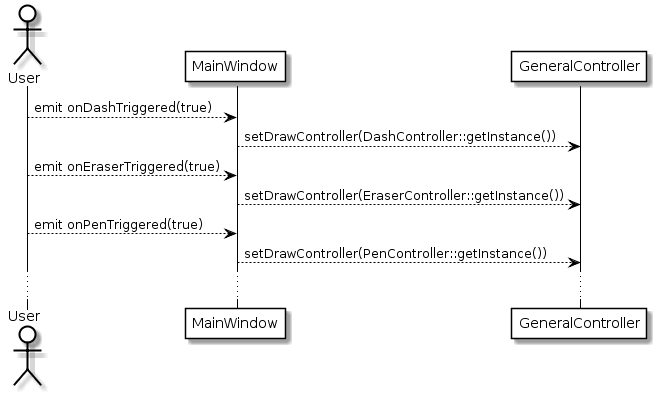
\includegraphics[scale=0.5]{images/tools-controllers-substitution.png}
\caption{Substitution des contrôleurs d'outils}
\end{figure}

La figure précédente résume parfaitement ce qui a été décrit plus tôt; l'utilisateur sélectionne un outil. Cette action a pour conséquence le déclenchement d'un événement adéquat au sein de l'interface graphique utilisateur. Celle-ci fait ensuite appel au contrôleur général pour mettre à jour le contrôleur d'outil courant.

\newpage

\subsection{Dessin}

Le concept de dessin correspond à n'importe quelle esquisse réalisée par l'utilisateur au moyen du stylet prévu et conçu à cet effet. Cela peut aller du simple point au milieu d'une surface à la modélisation en perspective du bâtiment du site de Cheseaux de la Haute École d'ingénierie et de gestion du canton de Vaud (Heig-VD).

\subsubsection{Vue virtuelle}

Bien qu'il soit prévu que le dessin esquissé soit projeté sur son support physique, le dessin logique du dessin doit être représenté sur le moniteur de l'utilisateur. En conséquence, une vue virtuelle du dessin doit être mise à disposition du système. Celui-ci fait entre autres appel aux contrôleurs de dessin pour y stocker logiquement et y retranscrire graphiquement les esquisses de l'utilisateur à la demande du contrôleur général.

\subsubsection{Structure logique}

La structure logique du dessin se base sur une structure de type \textit{bitmap}, c'est-à-dire une matrice où chaque élément de la matrice correspond à un pixel. La valeur stockée dans un tel élément consiste en la couleur de ce pixel. Cette couleur est représentée quant à elle par un code hexadécimal. En guise d'exemple, la figure suivante illustre une telle structure.

\begin{figure}[h]
\centering
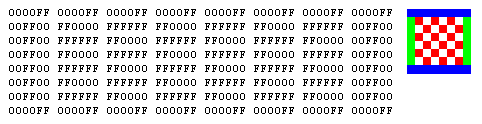
\includegraphics{images/drawing-structure.png}
\caption{Structure logique d'un dessin}
\end{figure}

\subsubsection{Représentation graphique}

La structure logique d'un dessin doit être traduite de manière à pouvoir obtenir une représentation graphique de celui-ci. Cette représentation graphique correspond au dessin affiché sur l'interface graphique utilisateur de l'application, sur le moniteur de l'utilisateur autrement dit.

\subsubsection{Projection}

La projection du dessin doit être réalisée par le biais d'un dispositif matériel adéquat. Dans le cadre de ce projet, il est préconisé de recourir à un projecteur lequel est censé être connecté à l'ordinateur. Le système d'exploitation de son côté veille à rediriger la représentation graphique du dessin vers la sortie matérielle faisant l'interface avec le périphérique de projection.

\newpage

\section{Stylet}

Cette section décrit la conception du stylet devant remplacer la souris de l'ordinateur pour dessiner sur un support physique. Sa conception ayant évolué en cours de projet, les différentes variantes y sont présentées. Chacune suit la même procédure de description. Les différents composants constituant ce stylet sont décrits de manière détaillée. Cela permet à tout un chacun de pouvoir reproduire cet outil en suivant les mêmes étapes de fabrication avec les mêmes composants voire des composants équivalents. Le prototype issu de la fabrication de l'outil de dessin est par la suite exposé. Finalement, le principe d'utilisation du stylet est présenté et commenté ce qui constitue un guide d'utilisation de celui-ci par la même occasion. Certains choix de conception y sont d'ailleurs justifiés.

\subsection{Modèle à une LED}

Le modèle à une LED du stylet a été défini lors de la définition du cahier des charges.

\subsubsection{Composants}

Le premier modèle du stylet est caractérisé par les composants suivants:

\begin{itemize}
\item[$\bullet$] Une LED rouge.
\item[$\bullet$] Un interrupteur.
\item[$\bullet$] Une résistance.
\item[$\bullet$] Une batterie.
\item[$\bullet$] Un boîtier.
\end{itemize}

\subsubsection{Fabrication}

\textit{TODO: décrire les étapes de fabrication du stylet (celles-ci devraient permettre à tout un chacun de pouvoir le créer à partir de zéro).}

\subsubsection{Prototype}

La figure suivante propose une ébauche de prototype du modèle à une LED du stylet:

\textit{TODO: inclure un schéma du prototype de stylet à une LED.}

\subsubsection{Fonctionnement}

\textit{TODO: décrire le fonctionnement interne du stylet.}

\subsubsection{Principe d'utilisation}

\textit{TODO: décrire le principe d'utilisation du stylet, c'est-à-dire ce qu'il faut faire exactement pour pouvoir dessiner (position du bras, disposition de la main et des doigts, appui sur l'interrupteur).}

\newpage

\subsection{Modèle à deux LEDs}

Le modèle à deux LED du stylet a été défini durant la première partie du projet. Il remplace le modèle à une LED.

\textit{TODO: expliquer et justifier la raison du changement de modèle.}

\subsubsection{Composants}

Le deuxième modèle du stylet est caractérisé par les composants suivants:

\begin{itemize}
\item[$\bullet$] Une LED rouge.
\item[$\bullet$] Une LED verte.
\item[$\bullet$] Un interrupteur.
\item[$\bullet$] Une résistance.
\item[$\bullet$] Une batterie.
\item[$\bullet$] Un boîtier.
\end{itemize}

\subsubsection{Fabrication}

\textit{TODO: décrire les étapes de fabrication du stylet (celles-ci devraient permettre à tout un chacun de pouvoir le créer à partir de zéro).}

\subsubsection{Prototype}

La figure suivante propose une ébauche de prototype du modèle à deux LEDs du stylet:

\textit{TODO: inclure un schéma du prototype de stylet à deux LEDs.}

\subsubsection{Fonctionnement}

\textit{TODO: décrire le fonctionnement interne du stylet.}

\subsubsection{Principe d'utilisation}

\textit{TODO: décrire le principe d'utilisation du stylet, c'est-à-dire ce qu'il faut faire exactement pour pouvoir dessiner (position du bras, disposition de la main et des doigts, appui sur l'interrupteur).}

\newpage

\subsection{Modèle laser}

Le modèle laser du stylet a été défini durant la deuxième partie du projet. Il remplace le modèle à deux LEDs.

\textit{TODO: expliquer et justifier la raison du changement de modèle.}

\subsubsection{Composants}

Le troisième modèle du stylet est caractérisé par les composants suivants:

\begin{itemize}
\item[$\bullet$] Une LED rouge.
\item[$\bullet$] Un interrupteur.
\item[$\bullet$] Une résistance.
\item[$\bullet$] Une batterie.
\item[$\bullet$] Un boîtier.
\end{itemize}

\subsubsection{Fabrication}

\textit{TODO: décrire les étapes de fabrication du stylet (celles-ci devraient permettre à tout un chacun de pouvoir le créer à partir de zéro).}

\subsubsection{Prototype}

La figure suivante propose une ébauche de prototype du modèle laser du stylet:

\textit{TODO: inclure un schéma du prototype de stylet laser.}

\subsubsection{Fonctionnement}

\textit{TODO: décrire le fonctionnement interne du stylet.}

\subsubsection{Principe d'utilisation}

\textit{TODO: décrire le principe d'utilisation du stylet, c'est-à-dire ce qu'il faut faire exactement pour pouvoir dessiner (position du bras, disposition de la main et des doigts, appui sur l'interrupteur).}

\newpage

\section{Environnement de dessin}

Cette section présente la conception de l'environnement de dessin. Ce travail de conception est nécessaire dans la mesure où le système ne peut être opérationnel et fonctionnel qu'à la seule condition de disposer d'un environnement de travail adéquat répondant à un certain nombre de pré-requis. Concrètement, il s'agit d'introduire le matériel nécessaire à sa mise en place, de décrire précisément celle-ci et de présenter un exemple d'environnement jugé idéal pour l'utilisation de l'application.

\subsection{Matériel requis}

Les points suivants constituent le matériel requis pour l'utilisation de l'application:

\begin{itemize}
\item[$\bullet$] Un prototype de stylet faisant office d'outil de dessin.
\item[$\bullet$] Une caméra permettant de traquer les mouvements du stylet.
\item[$\bullet$] Un projecteur vidéo permettant de retranscrire le dessin de l'utilisateur.
\item[$\bullet$] Un plan de travail permettant de dessiner.
\item[$\bullet$] Un support prévu pour la disposition de la caméra et du projecteur au-dessus du plan de travail.
\end{itemize}

Plusieurs remarques s'imposent quant à cette énumération du matériel requis. En premier lieu, la caméra mentionnée correspond à n'importe quel dispositif permettant de capturer des informations vidéos; il peut donc s'agir aussi bien d'une webcam, d'une micro-caméra d'un smartphone, d'une caméra intégrée à un ordinateur ou même d'une caméra professionnelle. La différence dans le choix de ce matériel influera toutefois la qualité du système de tracking du stylet. Par ailleurs, le projecteur vidéo n'est pas réellement obligatoire dans la mesure où l'utilisateur peut tout à fait dessiner sur un support donné. Il peut tout aussi bien constater le résultat de ses esquisses sur le moniteur de son ordinateur.

\subsection{Mise en place du matériel}

La mise en place du matériel requis est décrite par la procédure suivante:

\begin{enumerate}
\item Disposez le support de travail.
\item Posez le stylet sur le support de travail.
\item Placez la caméra au-dessus du support de travail.
\item Placez le projecteur vidéo au-dessus du support de travail.
\end{enumerate}

\subsection{Contraintes}

La procédure de mise en place n'est présentée ici qu'en guise de suggestion d'une disposition possible du matériel requis. Le but n'est pas d'imposer des contraintes matérielles et environnementales à l'utilisateur. Aussi, cette procédure peut effectivement être adaptée selon les besoins de l'utilisateur et/ou selon les possibilités que lui offre son environnement. L'important est de veiller à ce que le stylet demeure visible autant que possible dans le champ de vision de la caméra de manière à pouvoir le détecter et suivre ses mouvements de la manière la plus précise qui soit.

\subsection{Exemple d'environnement}

\begin{figure}[h]
\centering
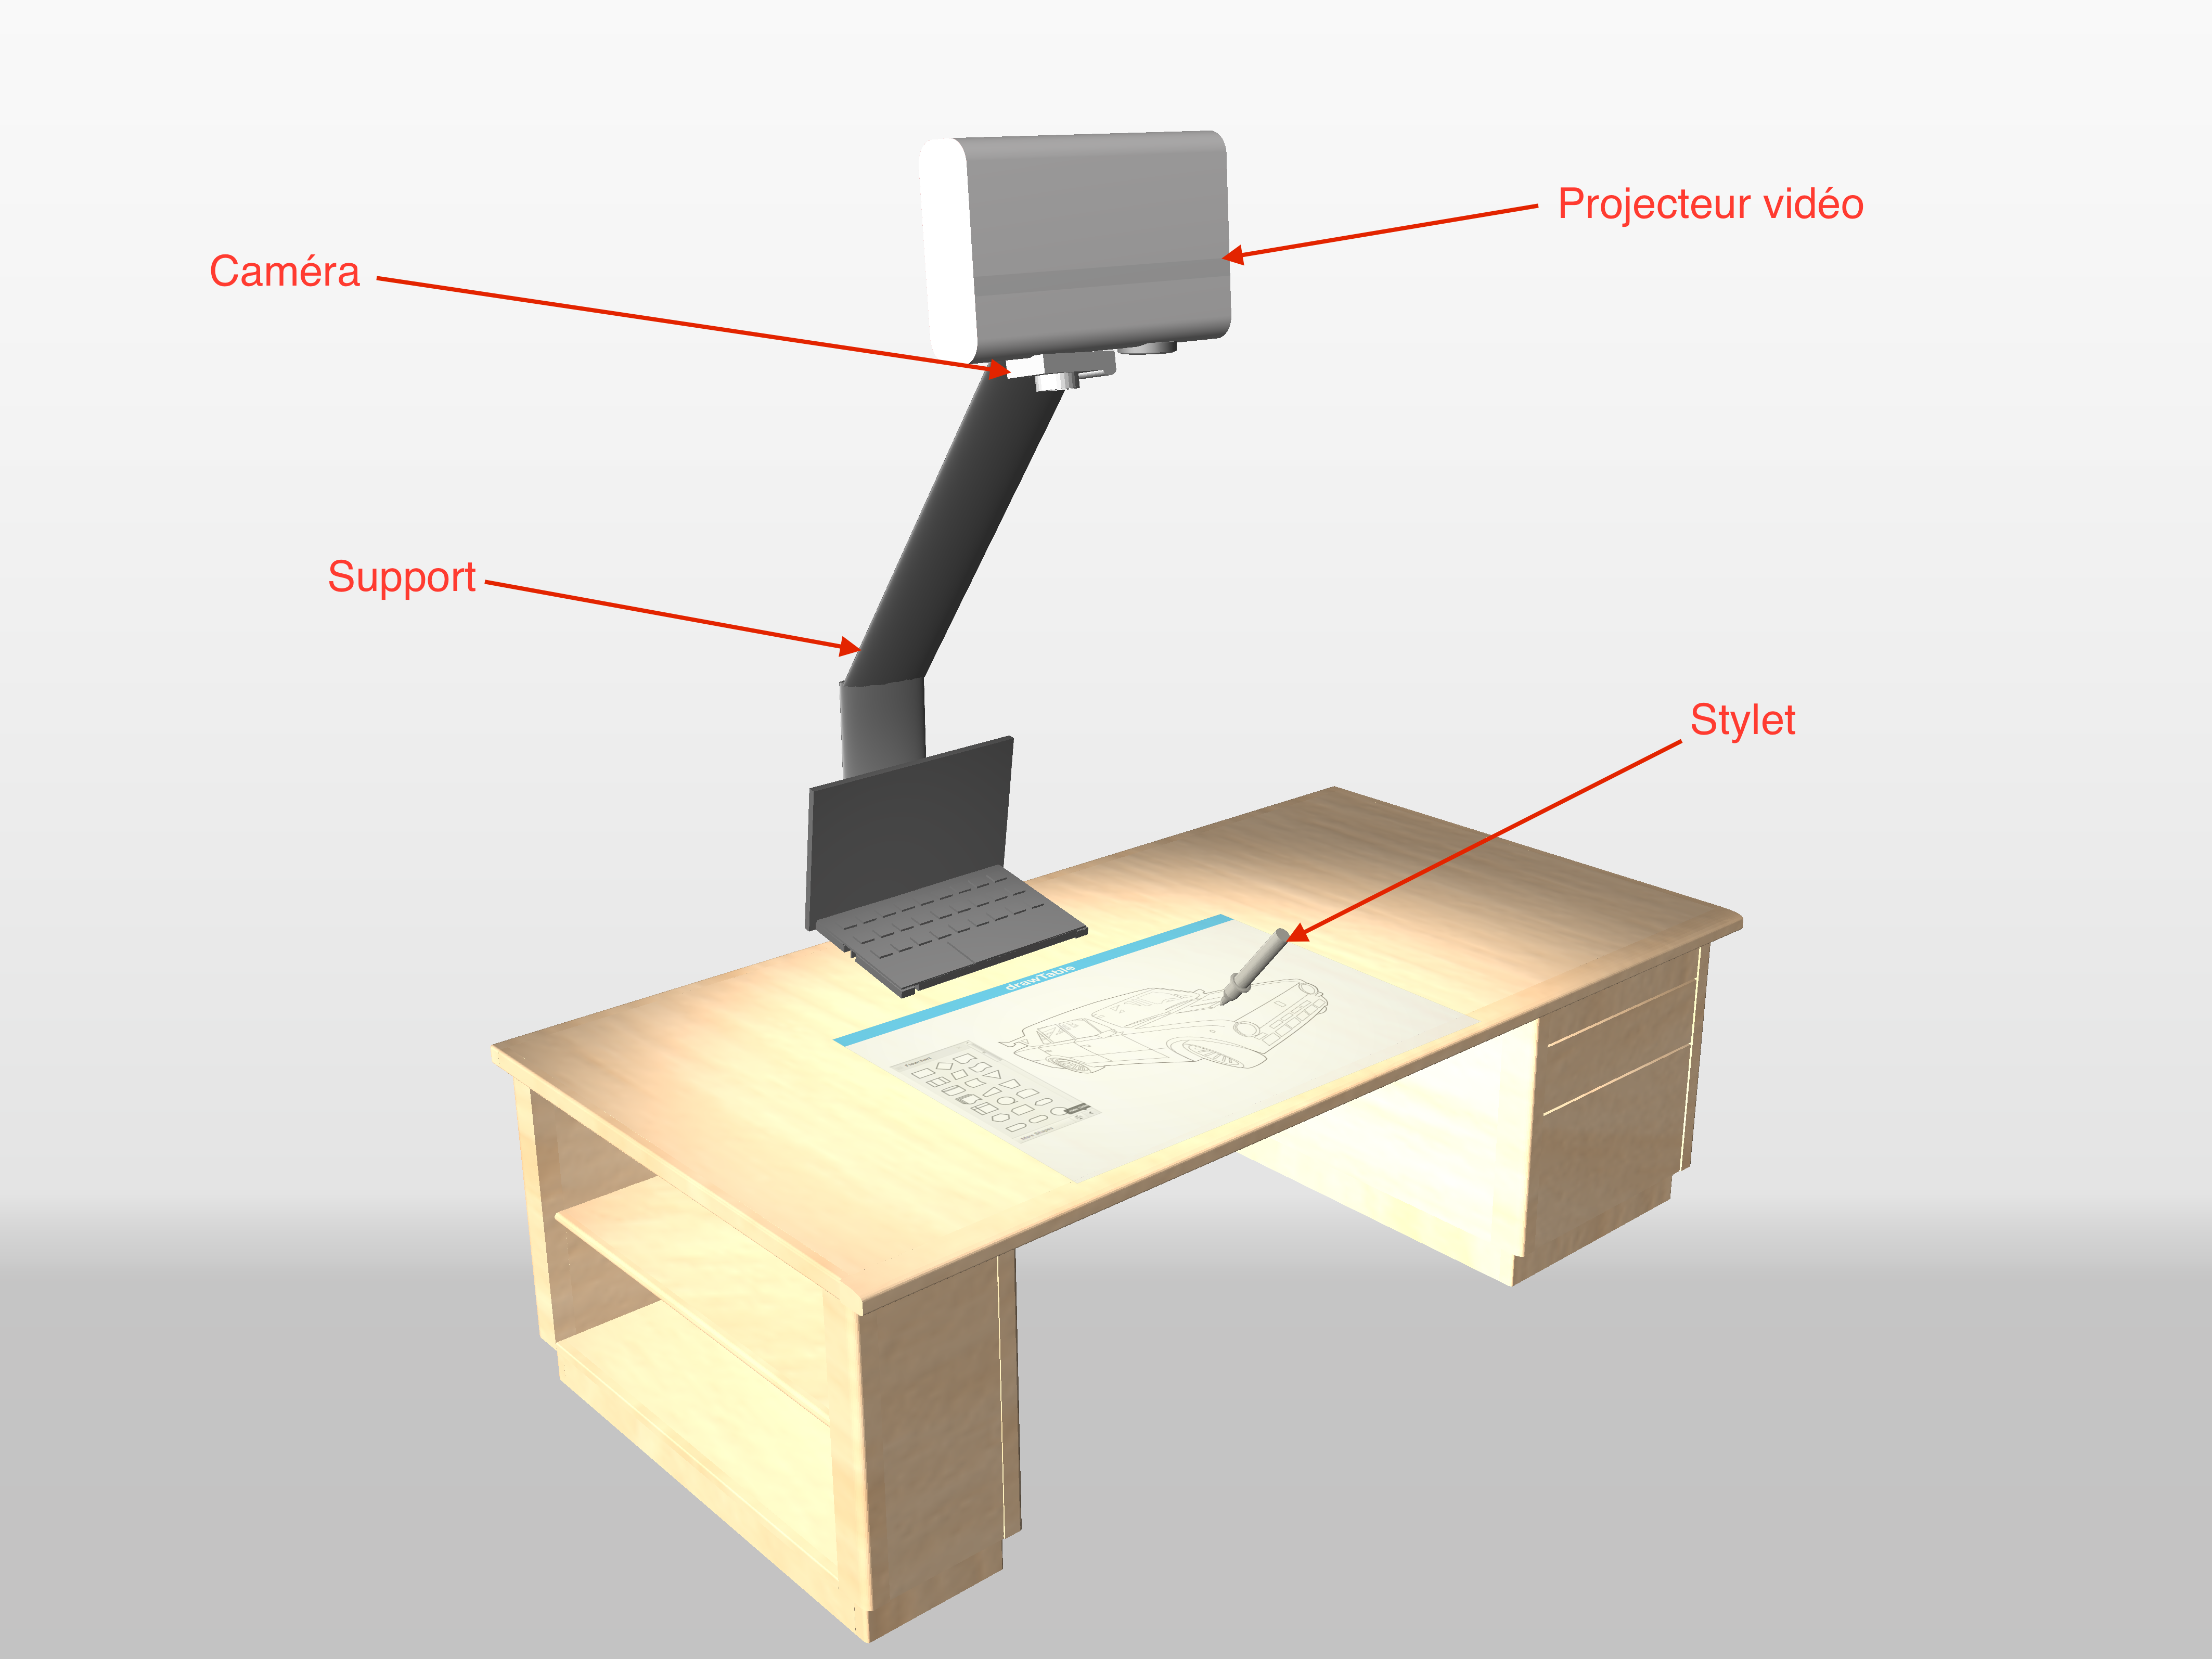
\includegraphics[angle=90, scale=0.15]{images/drawing-environment.png}
\caption{Exemple d'environnement de dessin - vue en perspective}
\end{figure}

\newpage

\begin{figure}[h]
\centering
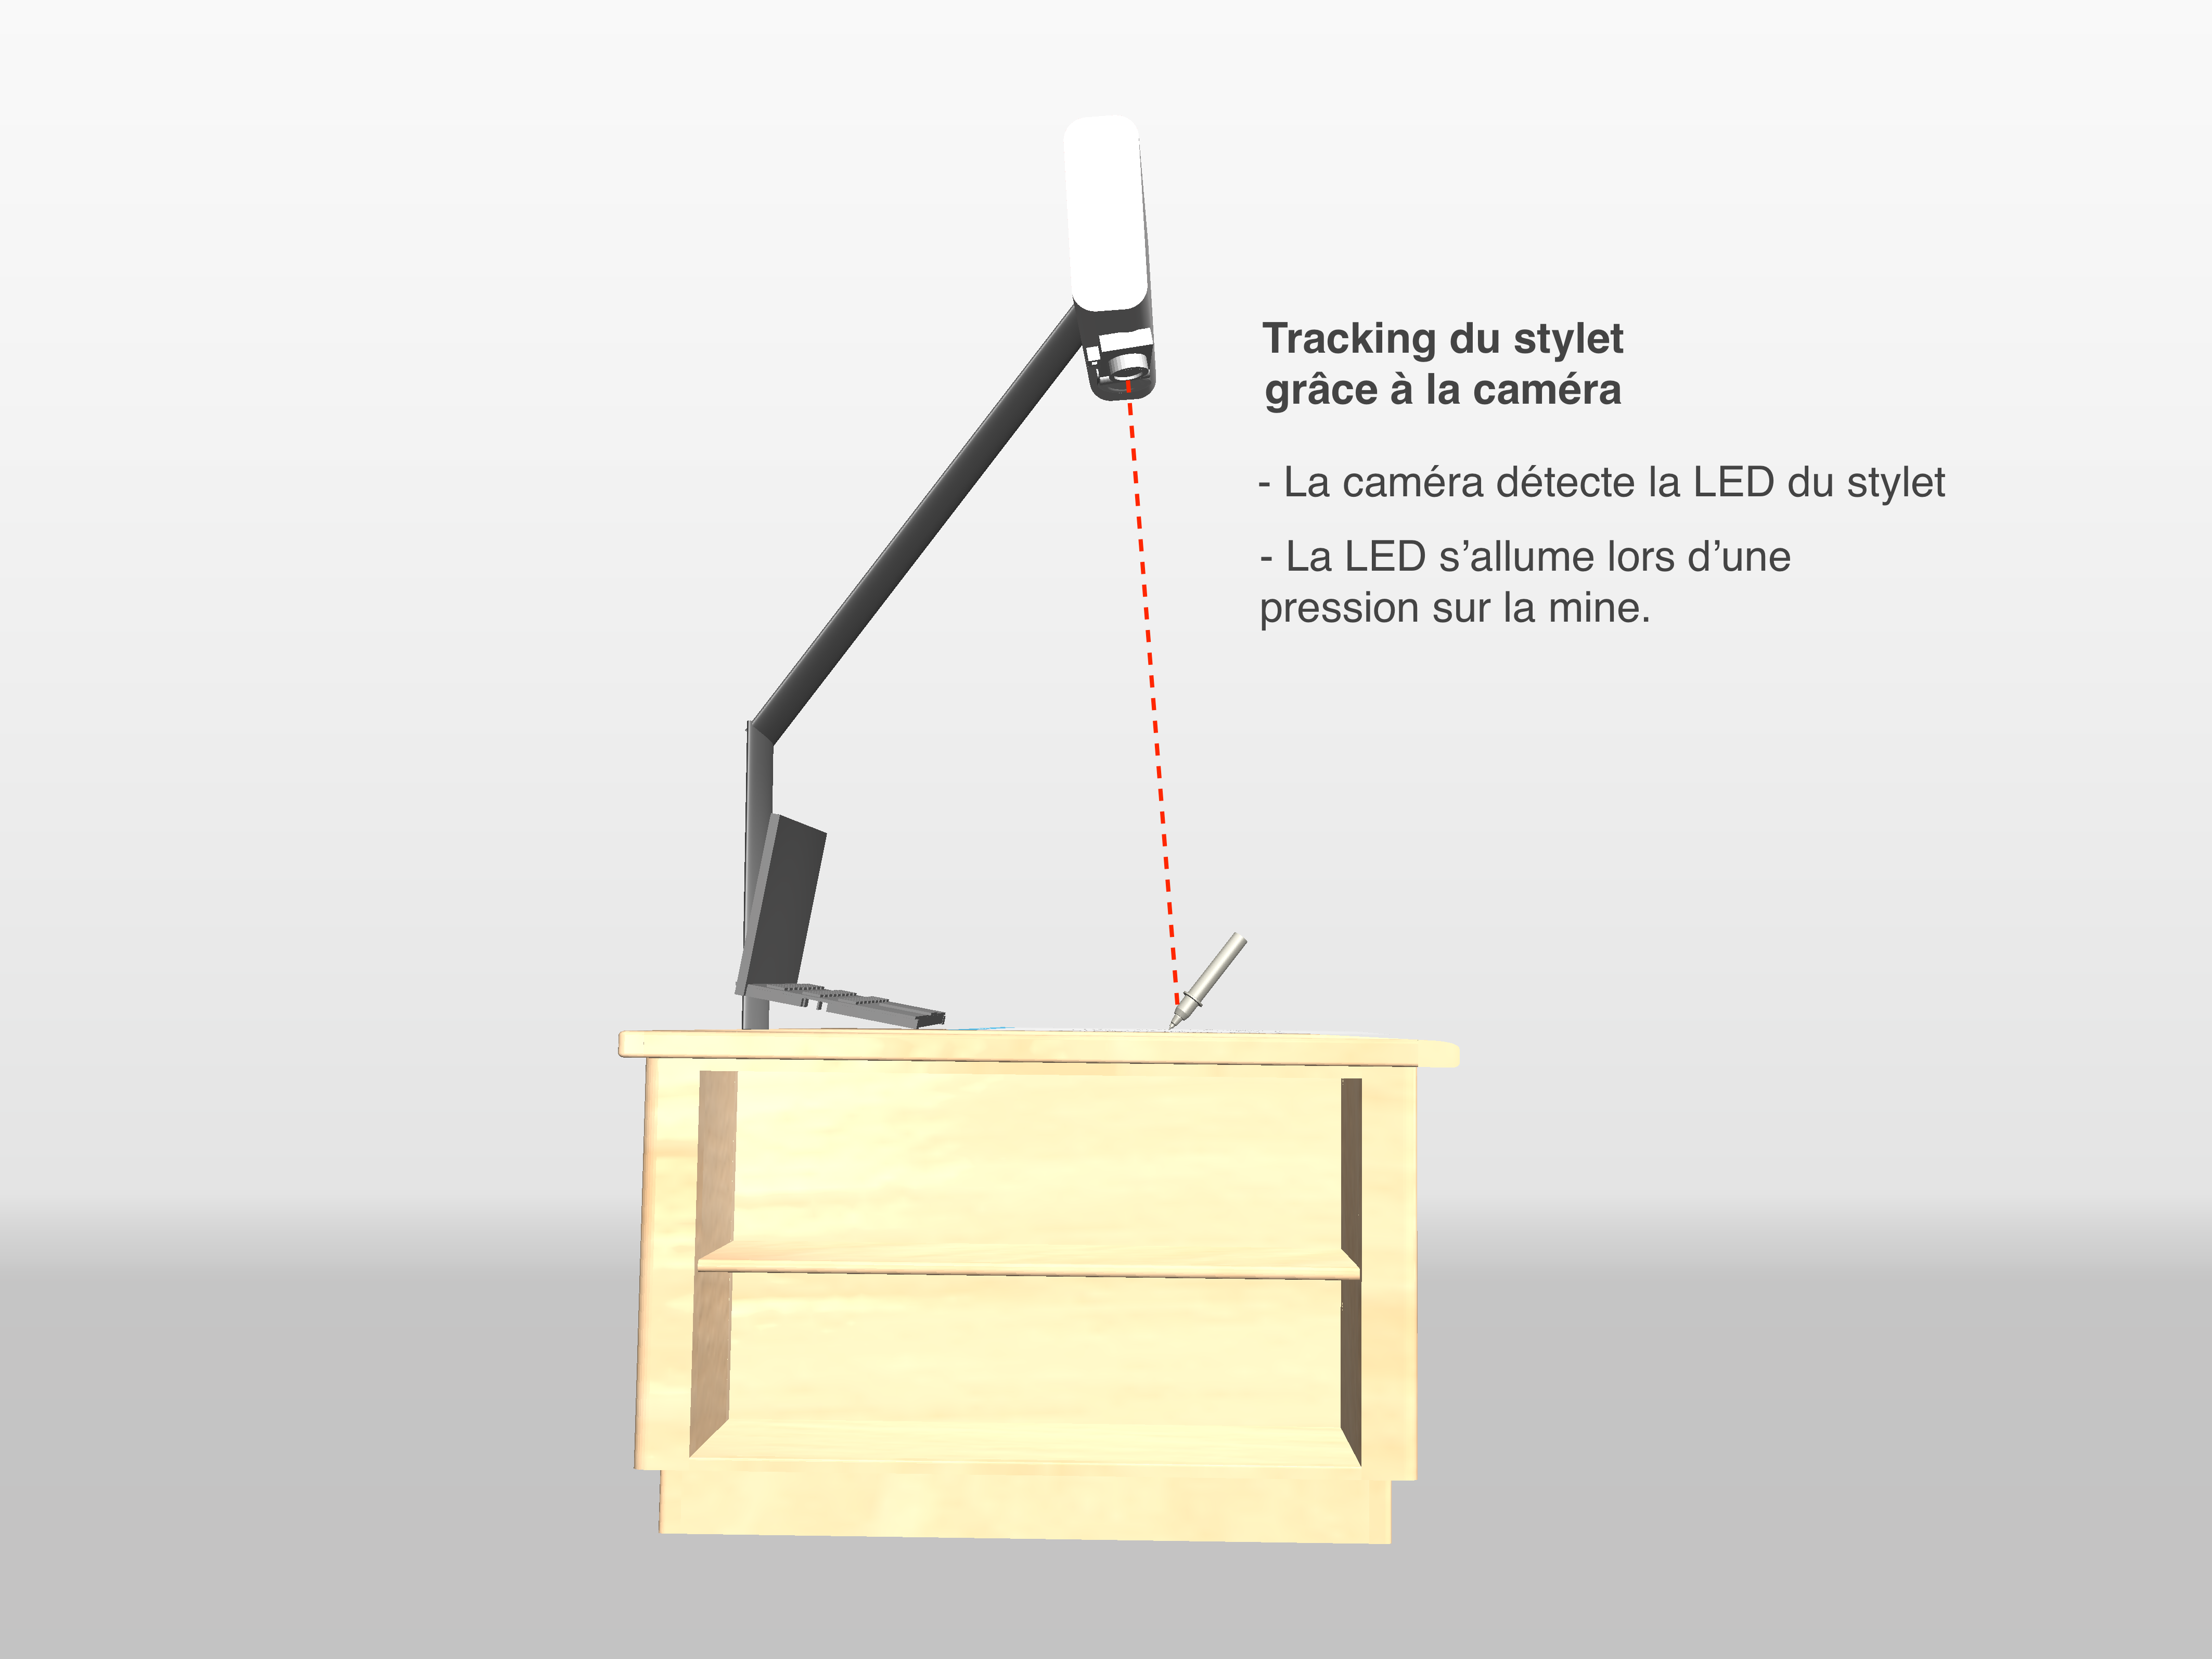
\includegraphics[angle=90, scale=0.15]{images/drawing-environment-side.png}
\caption{Exemple d'environnement de dessin - vue de gauche}
\end{figure}

%----------------------------------------------------------------------------------------
%	DESCRIPTION TECHNIQUE
%----------------------------------------------------------------------------------------

\chapter{Description technique}

\section{Vue d'ensemble des projets}

\section{Structure des projets}

\section{Patrons de conception}

\section{Librairies}

\section{Interface graphique utilisateur}

\subsection{Structure de l'interface utilisateur}

\subsection{Barre des menus}

\subsection{Barre d'outils}

\subsection{Zone de dessin}

\subsection{Ressources}

\section{Tracking}

\subsection{Système de détection}

\subsection{Mouvement du stylet}

\subsection{Déclenchement du dessin}

\subsection{Filtrage de couleurs}

\subsection{Précision du tracking}

\subsection{Contraintes de luminosité}

\newpage

\section{Dessin}

\subsection{Outils de dessin}

\subsubsection{Crayon}

\subsubsection{Gomme}

\subsection{Outils de formes}

\subsubsection{Trait}

\subsubsection{Rectangle}

\subsubsection{Cercle}

\subsection{Outils de couleurs}

\subsubsection{Palette de couleurs}

\subsection{Choix d'épaisseur}

\section{Interfaçage tracking-dessin}

\subsection{Communication inter-projet}

\subsubsection{Modèle des sockets}

\subsubsection{Protocole de communication}

\subsubsection{Structure des messages}

\subsection{Simulation et contrôle de la souris}

\section{Historique des actions}

\section{Sérialisation}

\section{Impression}

%----------------------------------------------------------------------------------------
%	PROCEDURE DE TESTS
%----------------------------------------------------------------------------------------

\chapter{Tests \& Validation}

\section{Stratégie de tests}

\section{Outils}

\section{Procédures de tests}

\section{Résultats}

%----------------------------------------------------------------------------------------
%	PROBLEMES CONNUS
%----------------------------------------------------------------------------------------

\chapter{Problèmes connus}

%----------------------------------------------------------------------------------------
%	CONCLUSION
%----------------------------------------------------------------------------------------

\chapter{Conclusion}

\section{Solution proposée}

\subsection{Fonctionnalités implémentées}

\subsection{Fonctionnalités manquantes}

\subsection{Propositions d'amélioration}

\section{Problèmes rencontrés}

\subsection{Problèmes organisationnels}

\subsection{Problèmes techniques}

\subsection{Problèmes de planification}

\section{Respect du planning}

\subsection{Planification initiale}

\subsection{Évolution}

\section{Déroulement du projet}

\subsection{Points positifs}

\subsection{Points négatifs}

\section{Synthèse}

%----------------------------------------------------------------------------------------
%	LISTINGS
%----------------------------------------------------------------------------------------

\lstlistoflistings

%----------------------------------------------------------------------------------------
%	APPENDIX
%----------------------------------------------------------------------------------------

\appendix

%----------------------------------------------------------------------------------------
%	CAHIER DES CHARGES
%------------------------------------------------------------------------------s----------

\chapter{Cahier des charges}

\section{Contexte}

Ce projet de groupe se déroule dans le cadre de la formation Bachelor HES de la Haute-Ecole d'Ingénierie et de Gestion du canton de Vaud. Il compte pour une unité d'enseignement du plan d'étude de l'orientation Informatique logiciel (IL) du département des Technologies de l'Information et de la Communication (TIC) de l'école. Il se réalise durant le cinquième semestre de l'année de formation 2015/16.

\section{Membres du groupe}

Les personnes suivantes constituent les membres du groupe de l'équipe de projet:

\begin{itemize}
\item[$\bullet$] Sacha Bron - \textit{Chef de groupe}
\item[$\bullet$] David Villa - \textit{Chef suppléant}
\item[$\bullet$] Paul Ntawuruhunga
\item[$\bullet$] Yassin Kammoun
\item[$\bullet$] Marc Pellet
\end{itemize}

\section{Objectif du projet}

L'objectif de ce projet est de concevoir un outil de dessin assisté par ordinateur permettant à l'utilisateur de réaliser ses dessins de la manière la plus naturelle possible. À terme, l'utilisateur dessinera directement sur sa table ou n'importe quelle autre surface plane à l'aide d'un stylet et son dessin sera projeté sur son plan de travail, donnant à l'utilisateur l'impression de dessiner avec un crayon et une feuille.

\section{Fonctionnalités principales}

Les fonctionnalités principales du projet sont les suivantes:

\begin{itemize}
\item[$\bullet$] Dessin à l’aide d’un stylet.
\item[$\bullet$] Projection de l’image sur le plan de travail.
\item[$\bullet$] Alignement de l’image avec la position du stylet.
\item[$\bullet$] Calibrage du stylet.
\item[$\bullet$] Plan de travail avec barre d'outils.
    \begin{itemize}
	\item Une barre d'outils sera projetée dans une zone du plan travail permettant à l'utilisateur de sélectionner un outil.
	\begin{itemize}
    \item[$\circ$] Outils de dessin: crayon, gomme.
	\item[$\circ$] Outils de forme: ligne droite, carré, cercle.
	\item[$\circ$] Outils de couleur: palette de couleurs.
	\item[$\circ$] Outils de choix d'épaisseur.
	\end{itemize}
    \end{itemize}
\item[$\bullet$] Annulation d’une action
    \begin{itemize}
	\item Une pile d'actions est enregistrée et un bouton dans la barre d'outils permet de remonter cette pile, annulant ainsi les dernières modifications apportées au dessin.
	\end{itemize}
\item[$\bullet$] Enregistrement et importation du dessin
	\begin{itemize}
	\item Possibilité d'enregistrer ou importer son dessin au format PNG.
	\end{itemize}
\end{itemize}

\section{Fonctionnalités supplémentaires}

Les fonctionnalités supplémentaires du projet sont les suivantes:

\begin{itemize}
\item[$\bullet$] Site vitrine.
\item[$\bullet$] Pipette.
\item[$\bullet$] Remplissage.
\item[$\bullet$] Rétablissement d'une action.
\end{itemize}

\section{Mockup}

La figure suivante illustre une ébauche de l'interface graphique utilisateur devant correspondre au plan de travail:

\begin{figure}[h]
\centering
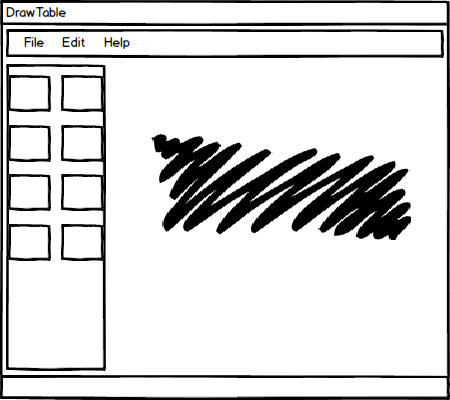
\includegraphics[scale=0.5]{images/ui.png}
\caption{Mockup de l'interface graphique utilisateur}
\end{figure}

L'interface graphique utilisateur est divisée en trois parties à savoir la barre des menus, la barre d'outils et la zone de dessin.

\section{Prototype du stylet}

Le prototype de stylet est conçu par le chef de projet. Sa conception nécessite les composants suivants:

\begin{itemize}
\item[$\bullet$] LED.
\item[$\bullet$] Un interrupteur.
\item[$\bullet$] Une résistance.
\item[$\bullet$] Une batterie.
\item[$\bullet$] Un boîtier.
\end{itemize}

La figure suivante propose une ébauche de prototype du stylet:

\newpage

\begin{figure}[h]
\centering
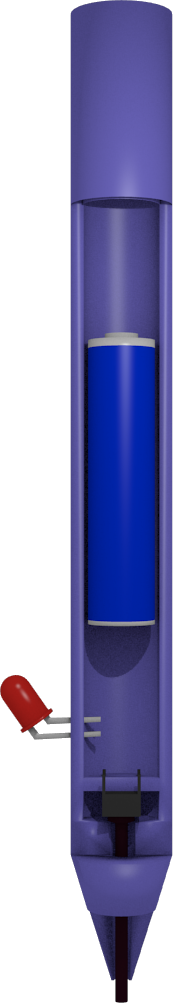
\includegraphics[scale=0.5]{images/stylus-first-design.png}
\caption{Prototype initial du stylet}
\end{figure}

\newpage

\section{Principe de fonctionnement}

Ce projet contient trois principales difficultés: la détection de contact du stylet sur la table, le suivi de la position du stylet (\textit{tracking}) et la précision de l'entier du système.

Pour cela nous avons imaginé un stylet muni d'une mine spéciale. Lors d'une pression sur le plan de travail, cette dernière presse sur un bouton qui enclenche une diode électroluminescente placée proche de la mine. Une caméra placée au-dessus du plan de travail filme la scène et envoie l'image au logiciel chargé de suivre la position de la mine du stylet en détectant cette LED.

Le programme de dessin récupère les coordonnées du stylet et les interprète de manière à pouvoir projeter le dessin sur le plan de travail à l'aide du projecteur vidéo.

L'application comportera différents threads: un thread de l'application sera consacré au tracking de la LED, un autre récupérera les coordonnées pour les interpréter sur le plan de travail en fonction de l'outil sélectionné.

\section{Public-cible}

L'application vise avant toute chose tout amateur de dessin souhaitant se passer d'une feuille.

\section{Technologies utilisées}

Les technologies utilisées pour le développement de l'application et le suivi du stylet sont les suivantes:

\begin{itemize}
\item[$\bullet$] Librairie OpenCV - Pour le suivi du stylet en temps réel.
\item[$\bullet$] Framework Qt - Pour l'interface graphique du plan de travail.
\end{itemize}

\section{Matériel requis}

Les points suivants constituent le matériel requis pour l'utilisation de l'application.

\begin{itemize}
\item[$\bullet$] Un prototype de stylet faisant office d'outil de dessin.
\item[$\bullet$] Une caméra permettant de traquer les mouvements du stylet.
\item[$\bullet$] Un projecteur vidéo permettant de retranscrire le dessin de l'utilisateur.
\item[$\bullet$] Un plan de travail permettant de dessiner.
\item[$\bullet$] Un support prévu pour la disposition de la caméra et du projecteur au-dessus du plan de travail.
\end{itemize}

\section{Plateformes supportées}

De par la nature du framework Qt, l'application est automatiquement multiplateforme; elle est donc supportée par les environnements usuels. Il s'agit entre autres des éditions Windows, des systèmes Mac OS X et des différentes distributions Linux. Un simple travail de recompilation du code source sur l'environnement désiré permet de disposer d'une version compatible de l'application.

\section{Déploiement}

\subsection{Installation de l'application}

Le déploiement de l'application suit la procédure standard des environnements supportés:

\begin{itemize}
\item[$\bullet$] Pour un environnement Windows, le déploiement se réalise par le biais d'un installateur.
\item[$\bullet$] Pour un environnement Mac OS X, le déploiement se réalise par le biais d'un fichier DMG.
\item[$\bullet$] Pour une distribution Linux (Arch), le déploiement se réalise par le biais d'un paquetage.
\end{itemize}

\subsection{Mise en place du matériel}

La mise en place du matériel requis est décrite par la procédure suivante:

\begin{enumerate}
\item  Disposez le support de travail.
\item  Posez le stylet sur le support de travail.
\item  Placez la caméra au-dessus du support de travail.
\item  Placez le projecteur vidéo au-dessus du support de travail.
\end{enumerate}

Les schémas suivants illustrent un environnement de travail idéal:

\newpage

\begin{figure}[H]
\centering
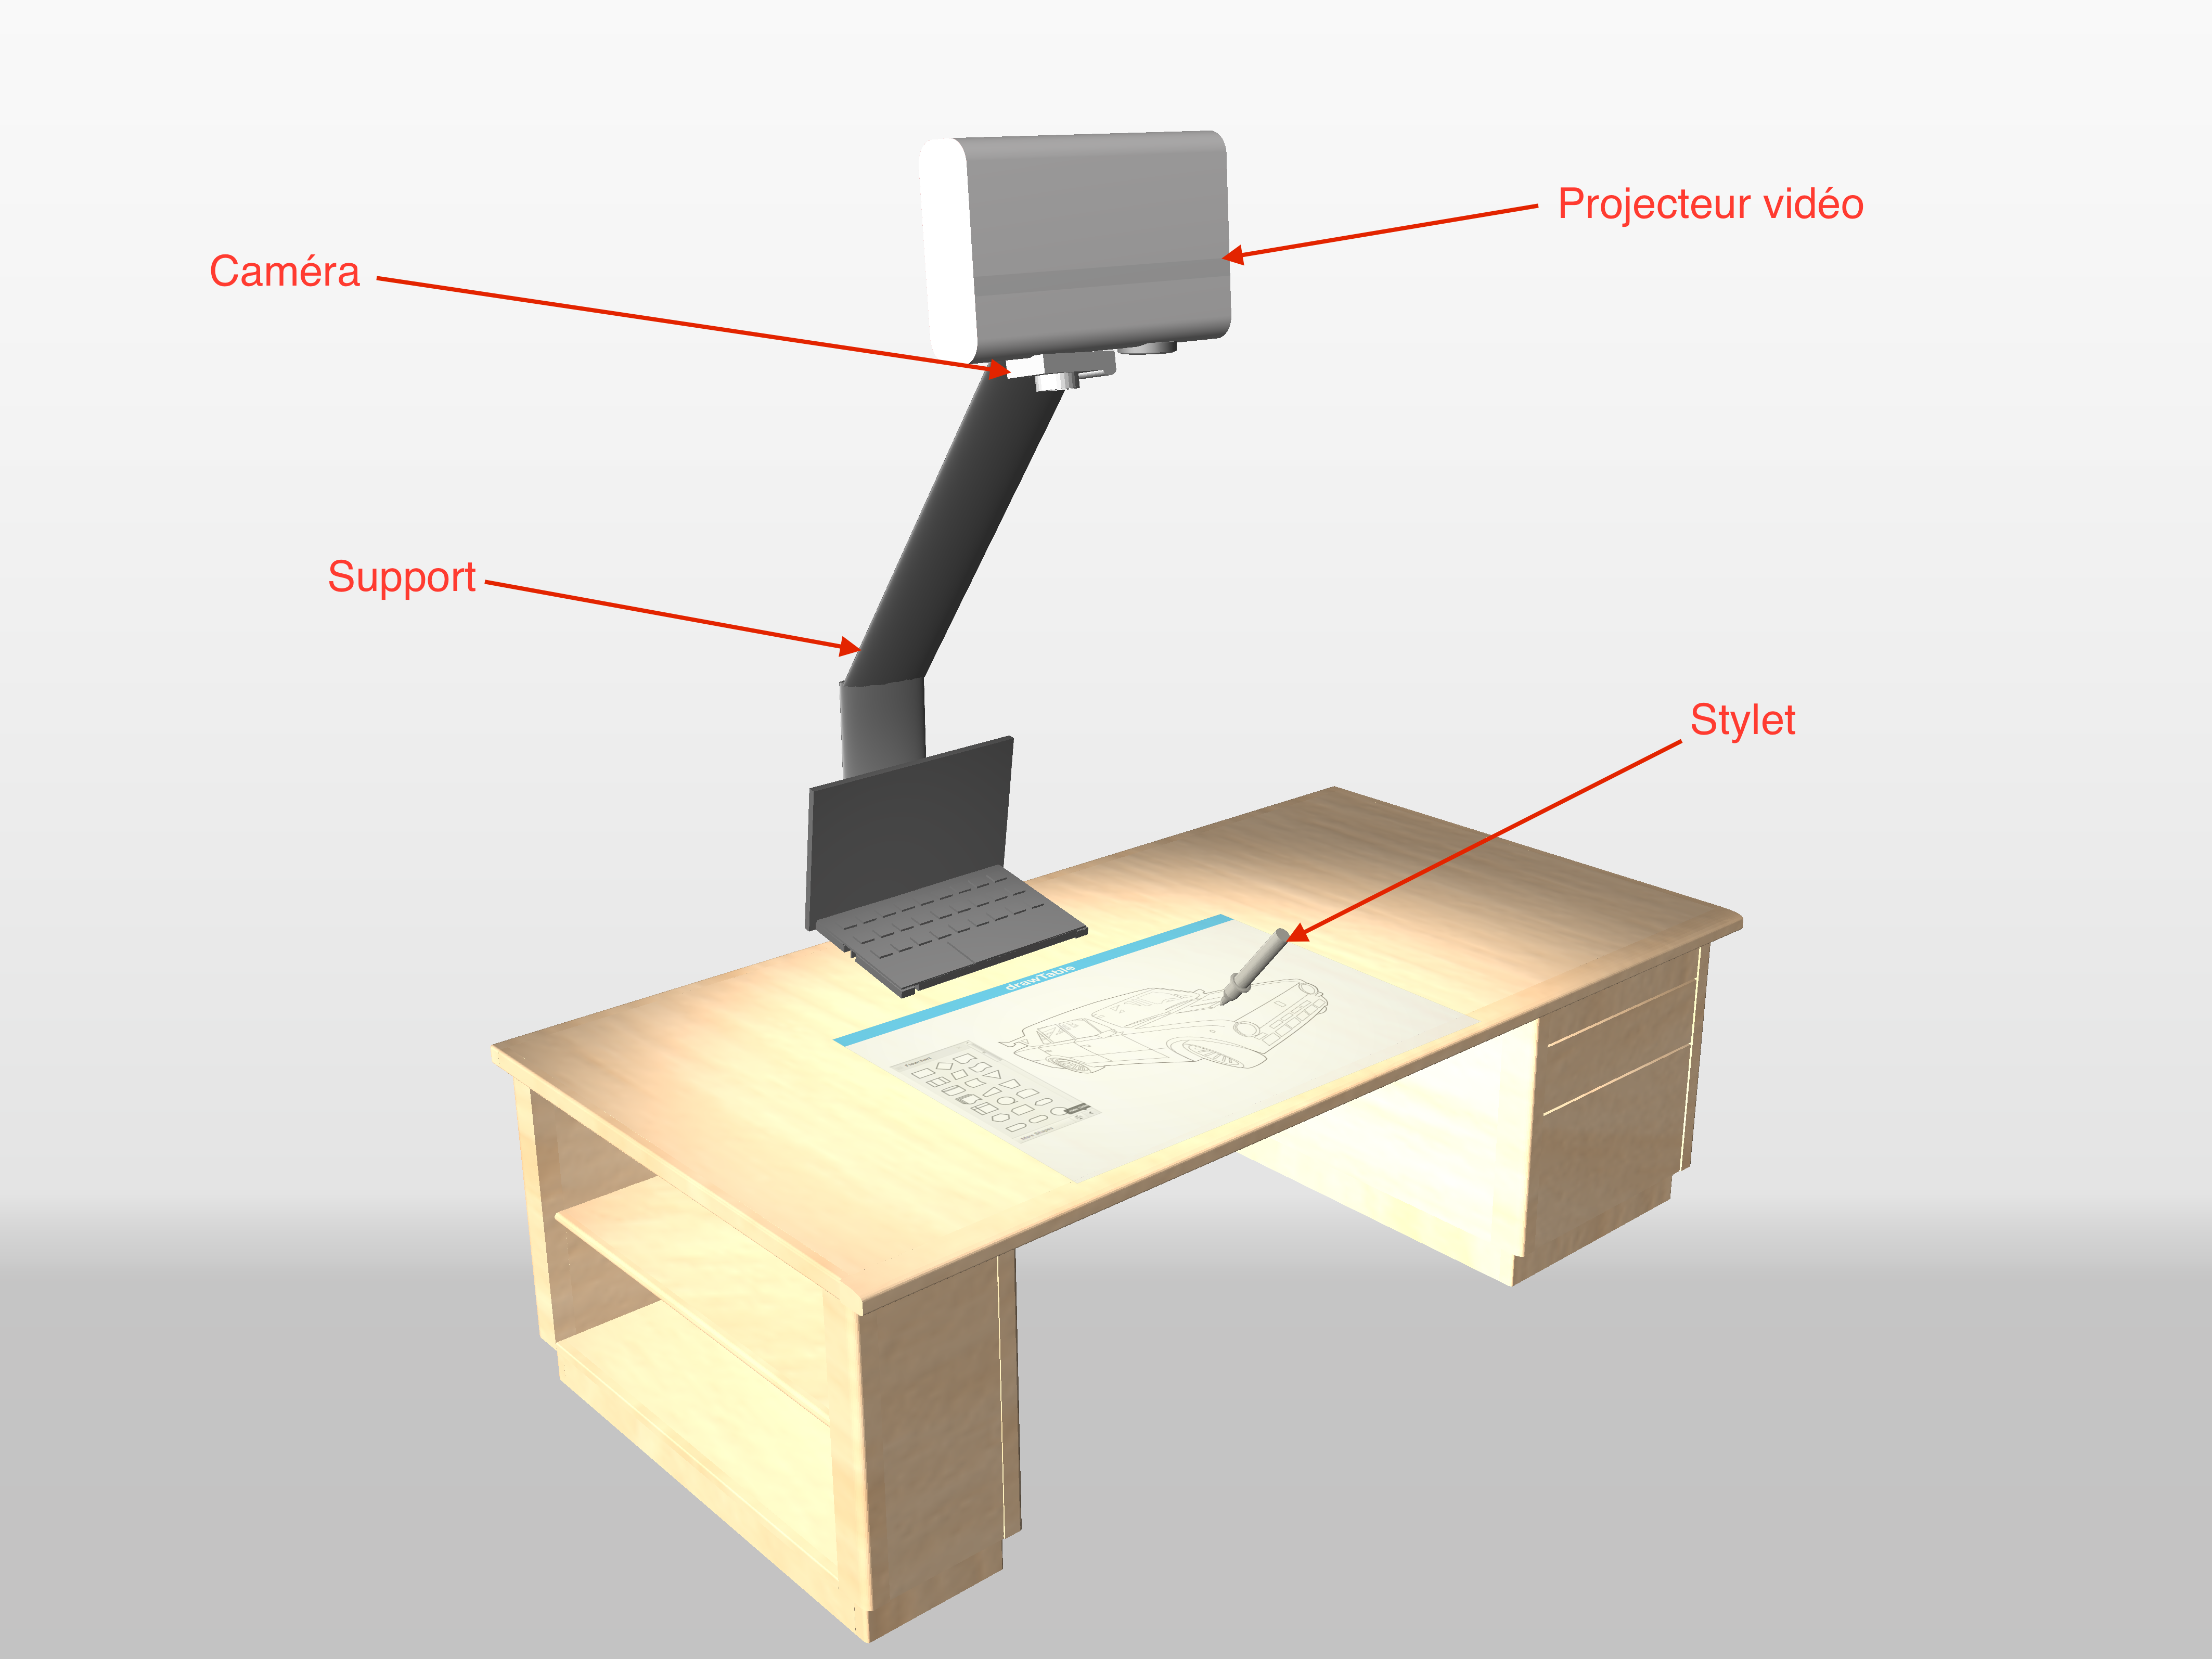
\includegraphics[angle=90, scale=0.15]{images/drawing-environment.png}
\caption{Vue en perspective d'un environnement idéal}
\end{figure}

\newpage

\begin{figure}[H]
\centering
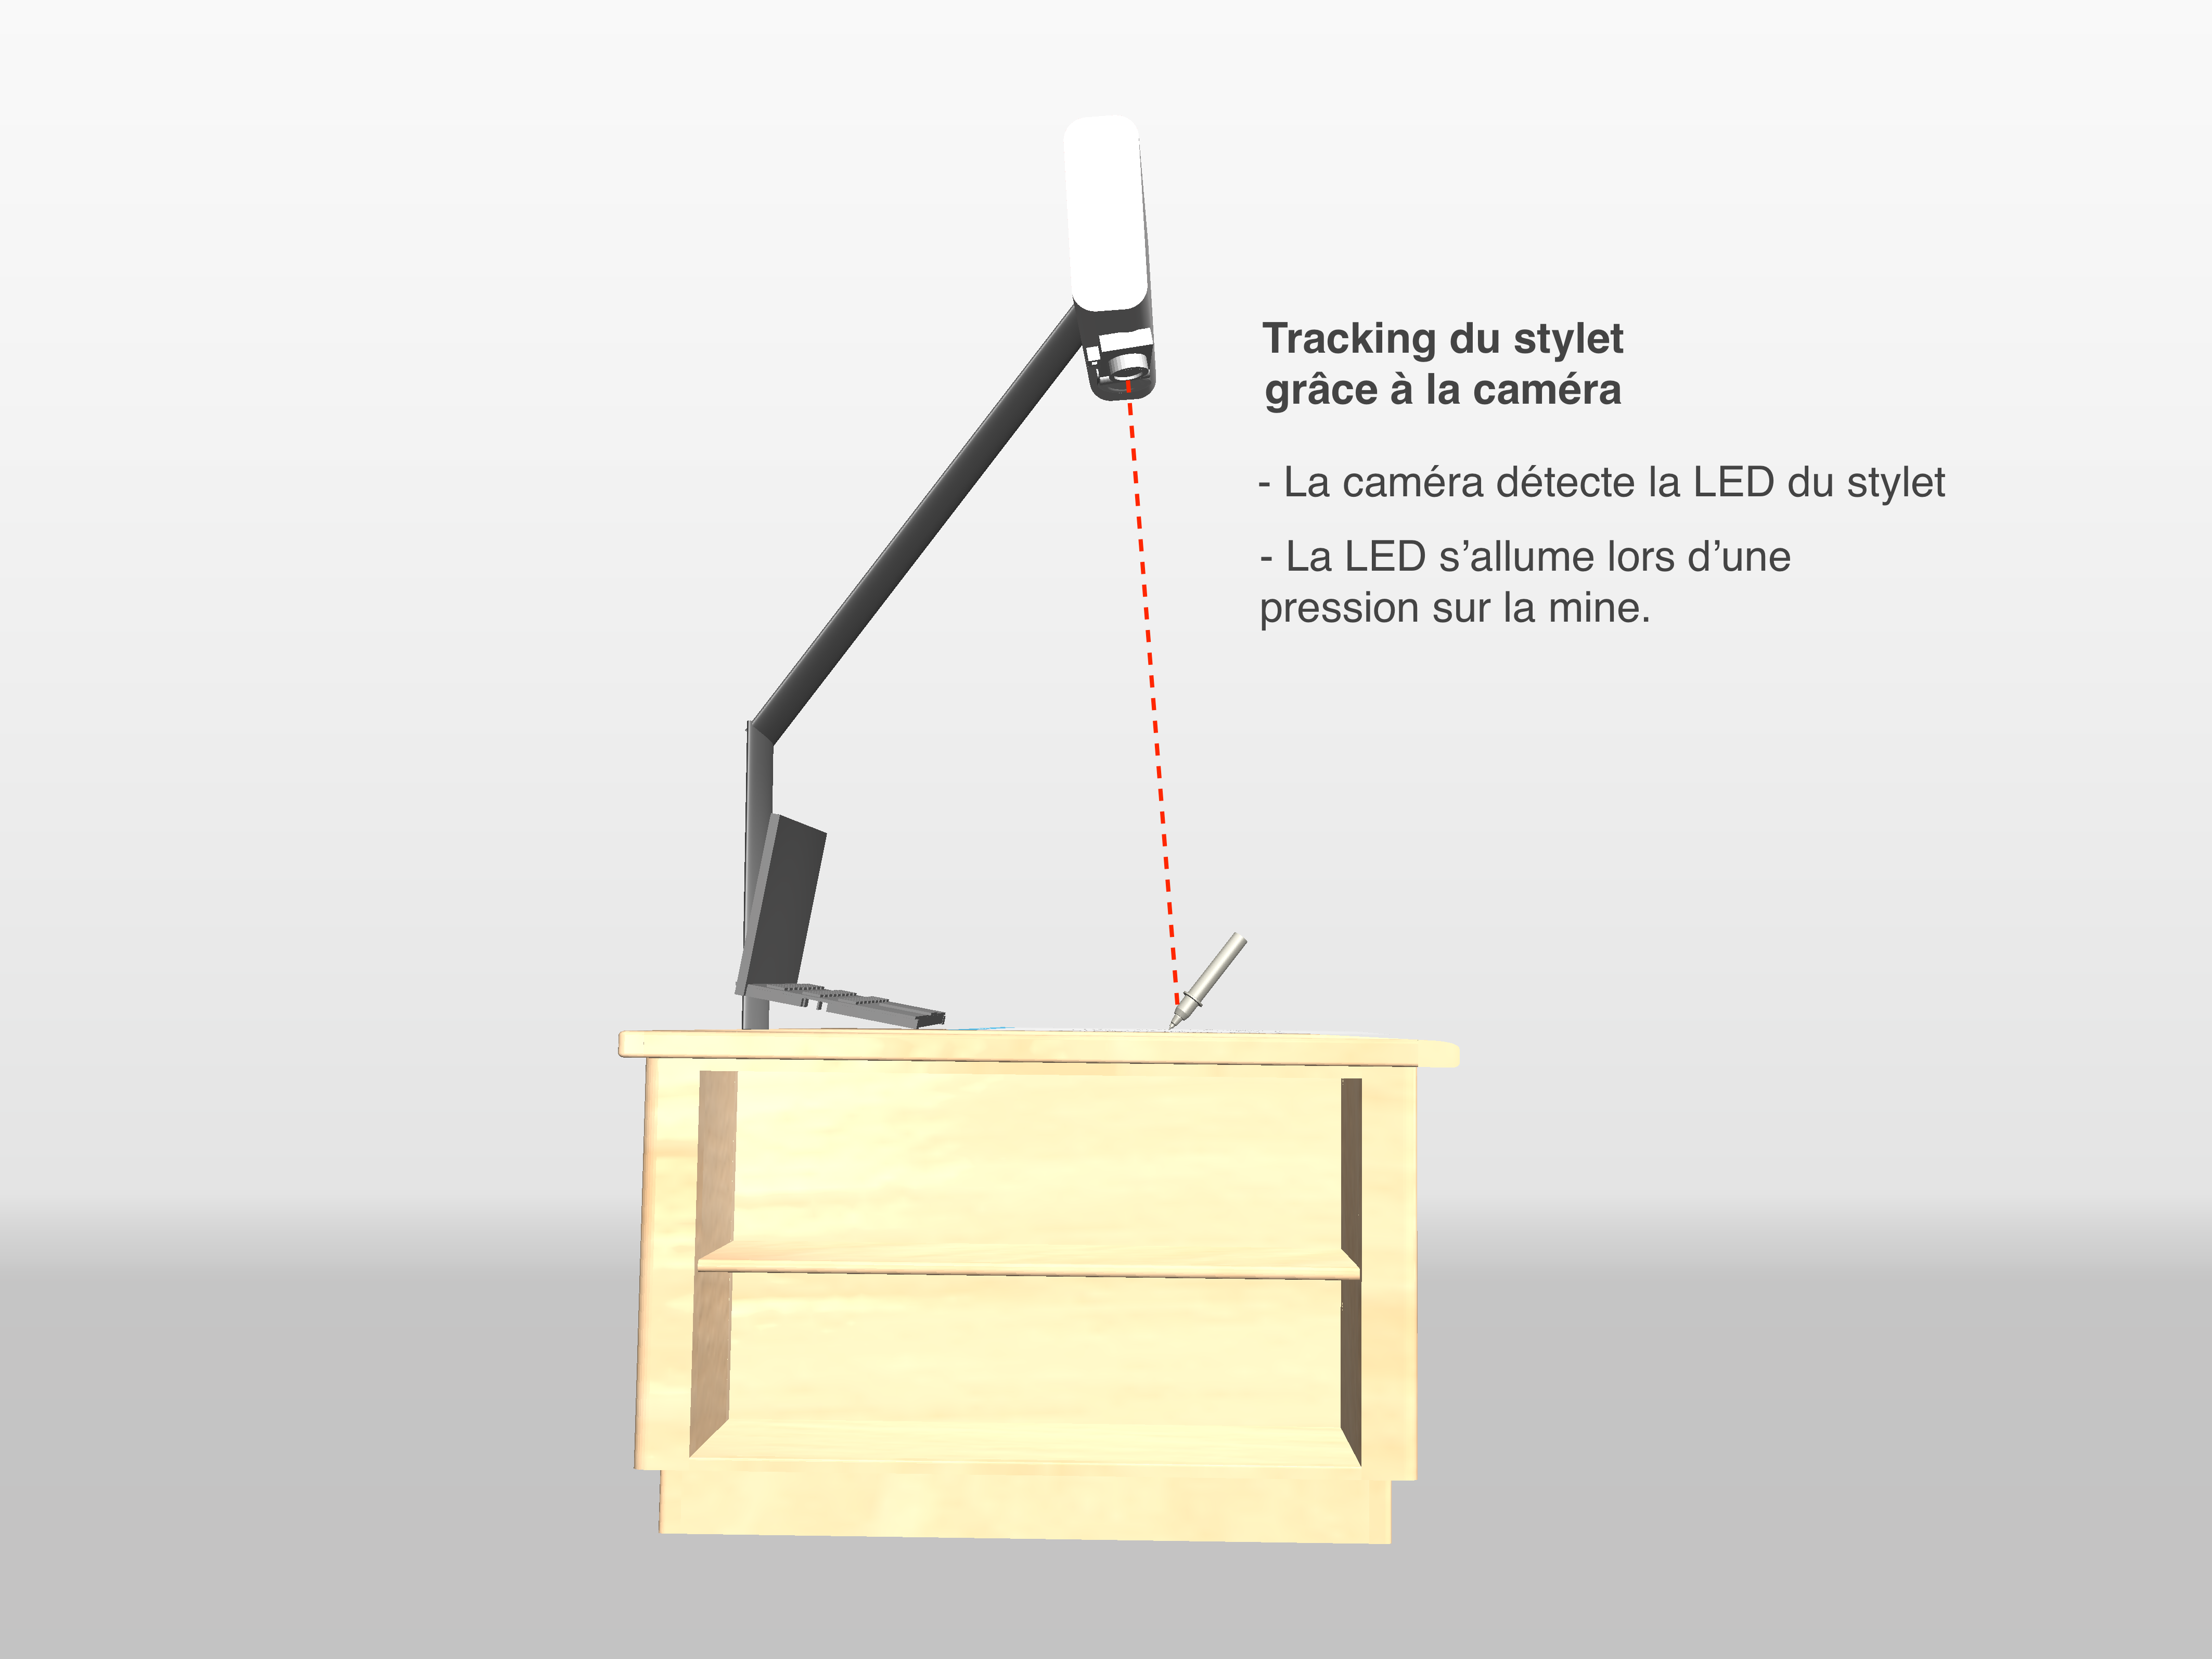
\includegraphics[angle=90, scale=0.15]{images/drawing-environment-side.png}
\caption{Vue de côté d'un environnement idéal}
\end{figure}

\newpage

\section{Déroulement du projet}

\subsection{Planification des tâches}

Le diagramme de Gantt qui suit présente la planification des tâches du projet:

\begin{figure}[H]
\centering
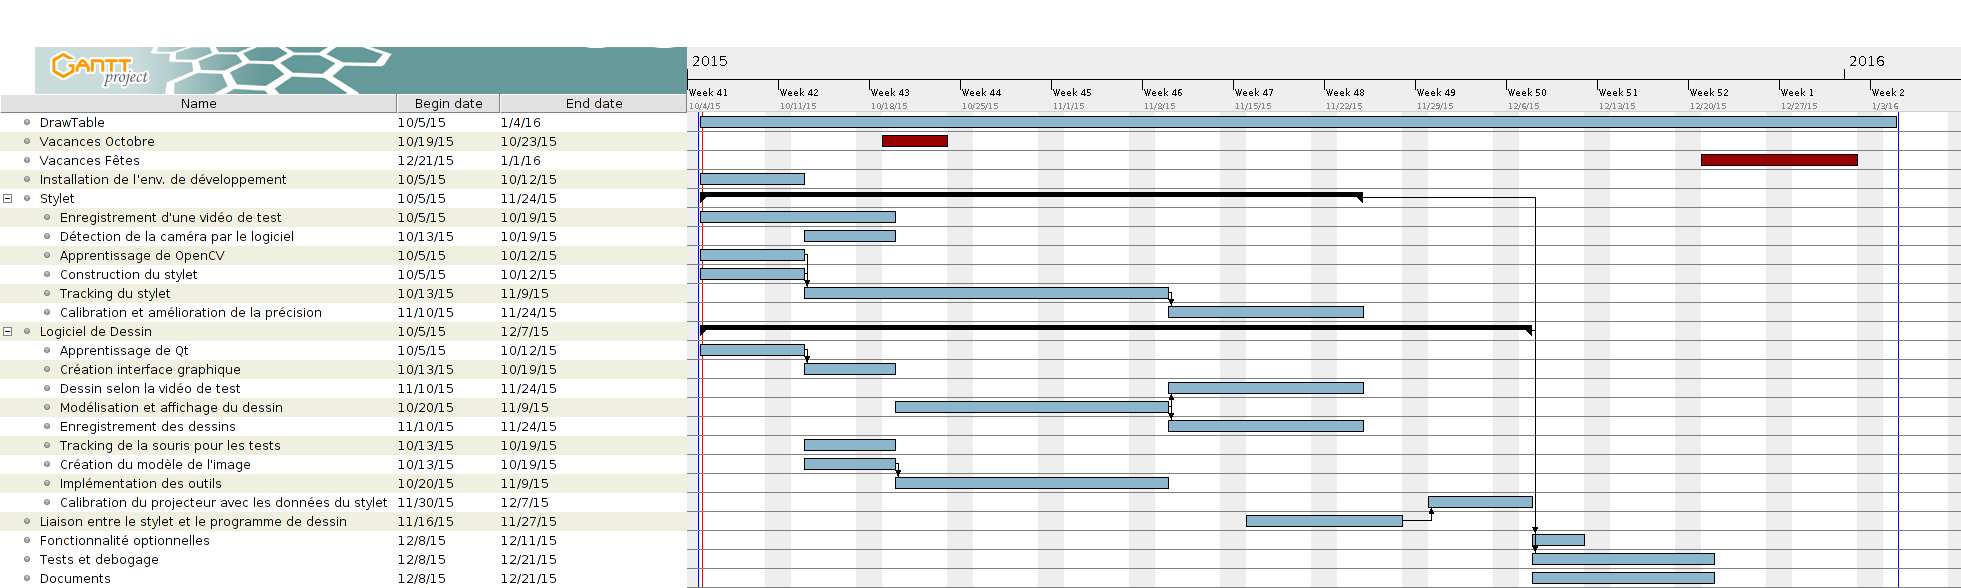
\includegraphics[angle=90, scale=0.3]{images/planification.png}
\caption{Planification initiale des tâches}
\end{figure}

\newpage

\subsection{Description des tâches}

Les points suivants constituent un bref descriptif des tâches du projet:

\begin{itemize}
\item[$\bullet$] Enregistrement d'une vidéo de test
    \begin{itemize}
	\item Afin de pouvoir tester les différents outils du logiciel de dessin avant que l'outil de tracking ne soit terminé, une vidéo contenant différents mouvements sera enregistrée.
	\end{itemize}
\item[$\bullet$] Apprentissage d'OpenCV
    \begin{itemize}
	\item Pour toutes les opérations de tracking du stylet, nous allons utiliser la librairie OpenCV. Il sera donc nécessaire de prendre le temps d’en apprendre les bases avant de se lancer à corps perdu dans l’implémentation.
	\end{itemize}
\item[$\bullet$] Construction d'un stylet
    \begin{itemize}
	\item Un stylet de notre propre création sera utilisé pour cette application, le matériel nécessaire à la fabrication de ce dernier est détaillé dans la description du prototype du stylet.
	\end{itemize}
\item[$\bullet$] Tracking du stylet
    \begin{itemize}
	\item A l’aide d’une caméra, nous détecterons les mouvements du stylet, il faudra donc récupérer ces informations et les transmettre au logiciel de dessin.
	\end{itemize}
\item[$\bullet$] Apprentissage de Qt
    \begin{itemize}
	\item Apprentissage des librairies Qt pour ce qui concerne principalement les interfaces graphiques et les librairies de dessin.
	\end{itemize}
\item[$\bullet$] Création de l’interface graphique
    \begin{itemize}
	\item Conception de l’interface graphique du logiciel. Celle-ci contiendra un menu permettant d’importer/exporter des images, d’un plan de travail sur lequel travailler ainsi qu’une boîte à outils contenant différentes fonctionnalités telles que le crayon, la gomme, une palette de couleurs, le choix de l’épaisseur du trait.
	\end{itemize}
\item[$\bullet$] Tracking intermédiaire de la souris
    \begin{itemize}
	\item Afin de permettre de tester le bon fonctionnement de l’implémentation des différents outils, ceci d’une manière accessible à tous les développeurs, il faut implémenter une fonctionnalité permettant de dessiner à l’aide de la souris.
	\end{itemize}
\item[$\bullet$] Création du modèle de l’image
    \begin{itemize}
	\item Conception et création du modèle qui sera utilisé par le logiciel pour représenter notre image.
	\end{itemize}
\item[$\bullet$] Implémentation des outils
    \begin{itemize}
	\item Implémentation des fonctionnalités obligatoires disponibles dans notre boîte à outils. Se référer à la description des fonctionnalités pour en connaître l'inventaire.
	\end{itemize}
\item[$\bullet$] Enregistrement des dessins
    \begin{itemize}
	\item Exportation de notre représentation de l’image en une image au format .PNG.
	\end{itemize}
\item[$\bullet$] Modélisation et affichage du dessin
    \begin{itemize}
	\item Implémentation des méthodes gérant l’affichage et la modélisation de notre image.
	\end{itemize}
\item[$\bullet$] Calibrage du projecteur avec les données du stylet
    \begin{itemize}
	\item Calibrage permettant de faire concorder la position de l’image projetée avec la position effective du stylet.
	\end{itemize}
\item[$\bullet$] Dessin selon la vidéo de test
    \begin{itemize}
	\item Utilisation d’une vidéo de test pré-enregistrée utilisant les méthodes de tracking implémentées permettant de tester les différents outils sans pour autant avoir le matériel à disposition.
	\end{itemize}
\item[$\bullet$] Liaison entre le stylet et le logiciel
    \begin{itemize}
	\item Liaison entre les données collectées par le système de tracking avec les méthodes d’affichage du logiciel.
	\end{itemize}
\end{itemize}

%----------------------------------------------------------------------------------------
%	JOURNAL DE TRAVAIL
%----------------------------------------------------------------------------------------

\chapter{Journal de travail}

\section{Semaine 1: 14 septembre 2015}

\section{Semaine 2: 21 septembre 2015}

\section{Semaine 3: 28 septembre 2015}

\section{Semaine 4: 5 octobre 2015}

\section{Semaine 5: 12 octobre 2015}

\section{Semaine 6: 26 octobre 2015}

\section{Semaine 7: 2 novembre 2015}

\section{Semaine 8: 9 novembre 2015}

\section{Semaine 9: 16 novembre 2015}

\section{Semaine 10: 23 novembre 2015}

\section{Semaine 11: 30 novembre 2015}

\section{Semaine 12: 7 décembre 2015}

\section{Semaine 13: 14 décembre 2015}

\section{Semaine 14: 4 janvier 2016}

\section{Semaine 15: 11 janvier 2016}

%----------------------------------------------------------------------------------------
%	PLANIFICATION
%----------------------------------------------------------------------------------------

\chapter{Planification}

\section{Planification initiale}

\begin{figure}[H]
\centering
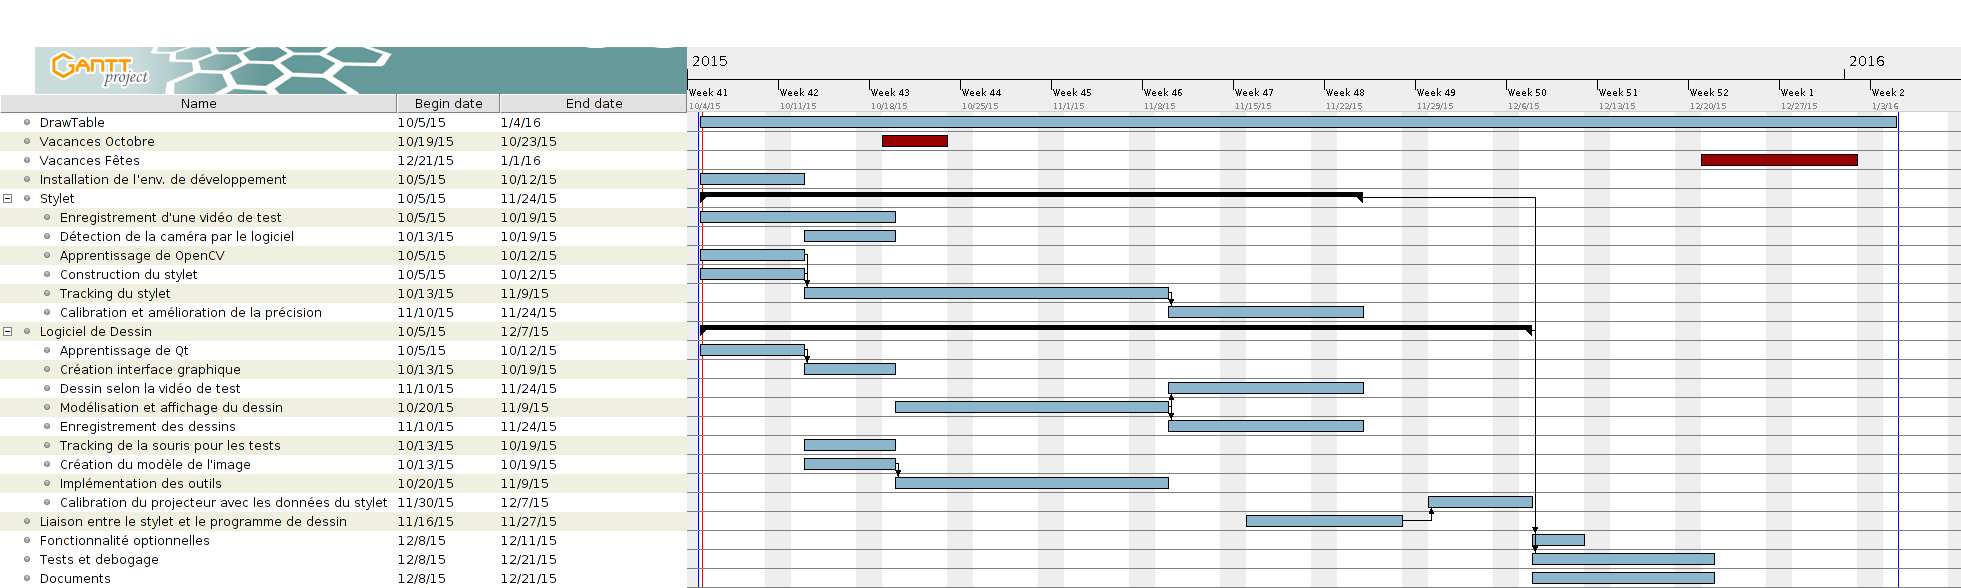
\includegraphics[angle=90, scale=0.35]{images/planification.png}
\caption{Planification initiale du projet}
\end{figure}

\newpage

\section{Planification finale}

\textit{TODO: définir la planification finale du projet avec Gantt Project.}

\end{document}